\documentclass{article}
\pdfpagewidth=8.5in
\pdfpageheight=11in

\usepackage{kr}

\usepackage{times}
\usepackage{soul}
\usepackage{url}
\usepackage[hidelinks]{hyperref}
\usepackage[utf8]{inputenc}
\usepackage[small]{caption}
\usepackage{graphicx}
\usepackage{amsmath}
\usepackage{amsthm}
\usepackage{booktabs}
\urlstyle{same}

\usepackage[backgroundcolor=lightgray]{todonotes}
\usepackage{listings}
\usepackage[linesnumbered,ruled,vlined]{algorithm2e}
\usepackage[capitalize,noabbrev]{cleveref}
\usepackage{microtype}
\usepackage{mathtools}
\usepackage{forest}
\usepackage{siunitx}
\usepackage{amsfonts}
\usepackage{pifont}
\usepackage[inline]{enumitem}

\usetikzlibrary{arrows.meta}

\newtheorem{theorem}{Theorem}
\newtheorem{fact}{Fact}
\theoremstyle{definition}
\newtheorem{definition}{Definition}
\newtheorem{example}{Example}

% TODO: 9 pages!!!

\pdfinfo{
/TemplateVersion (KR.2022.0, KR.2023.0, KR.2024.0)
}

\forestset{
  sn edges/.style={for tree={edge={-Latex}}}
}

\lstset{breaklines=true}
\lstset{language=C++,
        basicstyle=\ttfamily,
        stringstyle=\color{red},
        commentstyle=\color{green},
        breaklines=true,
        showstringspaces=false}

\crefname{line}{line}{lines}
\crefalias{formula}{equation}
\crefname{formula}{Clause}{Clauses}
\creflabelformat{formula}{#2\textup{(#1)}#3}

\DeclareMathOperator{\Dom}{Dom}
\DeclareMathOperator{\Doms}{Doms}
\DeclareMathOperator{\Vars}{Vars}
\DeclareMathOperator*{\argmin}{argmin}
\DeclareMathOperator{\GDR}{GDR}

\newcommand{\cmark}{\ding{51}}
\newcommand{\xmark}{\ding{55}}

\newcommand{\expr}{\mathtt{expr}}
\newcommand{\Ctwo}{$\mathsf{C}^{2}$}
\newcommand{\FO}{$\mathsf{FO}$}
\newcommand{\UFO}{$\mathsf{UFO}^{2} + \mathsf{EQ}$}

\newcommand{\Cranetwo}{\textsc{Crane}~2}

\SetKwFunction{Crane}{Compile}
\SetKwFunction{Propagate}{Propagate}
\SetKwFunction{FindBaseCases}{FindBaseCases}

\title{Towards Efficient First-Order Model Counting}

% TODO: check if this follows the formatting guidelines
\author{%
Ananth K. Kidambi$^1$\and
Guramrit Singh$^1$\and
Paulius Dilkas$^2$\and
Kuldeep S. Meel$^3$ \\
\affiliations
$^1$Indian Institute of Technology Bombay, India\\
$^2$National University of Singapore, Singapore\\
$^3$University of Toronto, Canada\\
\emails
\{210051002, 210050061\}@iitb.ac.in,
paulius.dilkas@nus.edu.sg,
meel@cs.toronto.edu
}

\begin{document}

\maketitle

\begin{abstract}
\end{abstract}

\section{Introduction}

\todo[inline,caption={}]{
  \begin{itemize}
    \item describe which compilation rules are currently greedy or non-greedy
    \item my agenda has a plan for proving completeness for $\mathbf{C}^{2}$
    \item Can I prove that my domain recursion can always simulate the domain
          recursion of \textsc{ForcLift}?
  \end{itemize}
}

\paragraph{Papers to cite.}
\begin{itemize}
  \item original domain recursion~\cite{DBLP:conf/nips/Broeck11}
  \item recent overview paper~\cite{DBLP:conf/ijcai/Kuzelka23}
  \item conjecturing recurrence relations~\cite{DBLP:conf/ilp/BarvinekB0ZK21}
  \item algorithms
  \begin{itemize}
    \item \textsc{ForcLift}~\cite{DBLP:conf/ijcai/BroeckTMDR11}
    \item \textsc{Crane}~\cite{DBLP:conf/kr/DilkasB23}
    \item \textsc{FastWFOMC}~\cite{DBLP:conf/uai/BremenK21}
    \item approximate~\cite{DBLP:conf/ijcai/BremenK20}
  \end{itemize}
  \item liftable fragments (TODO: perhaps good sources of benchmarks?)
  \begin{itemize}
    \item \Ctwo~\cite{DBLP:journals/jair/Kuzelka21}
    \item tree axioms~\cite{DBLP:journals/ai/BremenK23}
    \item linear order axioms~\cite{DBLP:conf/aaai/TothK23}
  \end{itemize}
  \item applications
  \begin{itemize}
    \item extensions to
          sampling~\cite{DBLP:conf/aaai/WangB0K22,DBLP:conf/lics/WangP0K23}
    \item discovery of combinatorial
          sequences~\cite{DBLP:conf/ijcai/SvatosJT0K23}
  \end{itemize}
\end{itemize}

% TODO: make sure to not call \Crane2 \textsc{Crane}

\paragraph{Changes to the compilation process.}
\begin{itemize}
  \item We make the FCGs satisfy the following property. For every domain
        $\Delta$, for every directed path $P$ without Ref nodes, the number of
        atom counting or (generalised) domain recursion or independent partial
        grounding operations on $\Delta$ on $P$ is at most one.
  \item when checking whether recursion is possible between a source and a
        target formula, the target formula (maybe the source formula as well?)
        must not include a domain as well as its subdomain. This might be
        equivalent to the formula being `unshattered'. Such formulas could be
        seen as transitory, and allowing such recursive calls leads to FCGs that
        I cannot make sense of.
\end{itemize}

\paragraph{Proof of correctness (leave for later).}
\begin{enumerate}
  \item Define what it means for a formula to be \emph{consistent}.
        \begin{itemize}
          \item The formula (including the mapping of constants to their
                domains) does not mention a domain together with its subdomain
                (i.e., all mentioned domains are pairwise disjoint).
                Specifically, we can't have a subdomain together with its parent
                domain or a subdomain together with a constant that belongs to
                its parent domain.
          \item The target of \texttt{Ref} must also be a consistent formula.
          \item The initial formula is consistent by definition.
        \end{itemize}
  \item Aim to show that \Cranetwo{} works correctly on all consistent formulas.
  \item Prove that, whenever some compilation rule makes the formula $\phi$
        inconsistent, greedy compilation rules will make $\phi$ consistent again
        before $\phi$ encounters non-greedy compilation rules that depend on
        $\phi$ being consistent.
        \begin{itemize}
          \item In particular, prove that shattering and unit propagation will
                always eliminate the parent domain of the domains introduced by
                atom counting.
          \item Constraint removal only applies when it can eliminate the parent
                domain entirely.
          \item Prove this for a particular assumption about which compilation
                rules are set to be greedy. For the greedy algorithm, although
                all rules are applied in a greedy manner, we still assume that
                greedy rules will be applied before non-greedy rules.
        \end{itemize}
  \item In particular, independent partial groundings and atom counting are the
        two classical rules that require the formula to be shattered.
  \end{enumerate}

 % TODO: Crane2 uses itself instead of Crane. Not really. By 'Crane', here I
 % mean the process of turning logical formulas into equations. Later on, I use
 % 'Crane' to refer to Crane2. Maybe rename this use of 'Crane' to something
 % else?
\begin{figure*}[t]
  \centering
  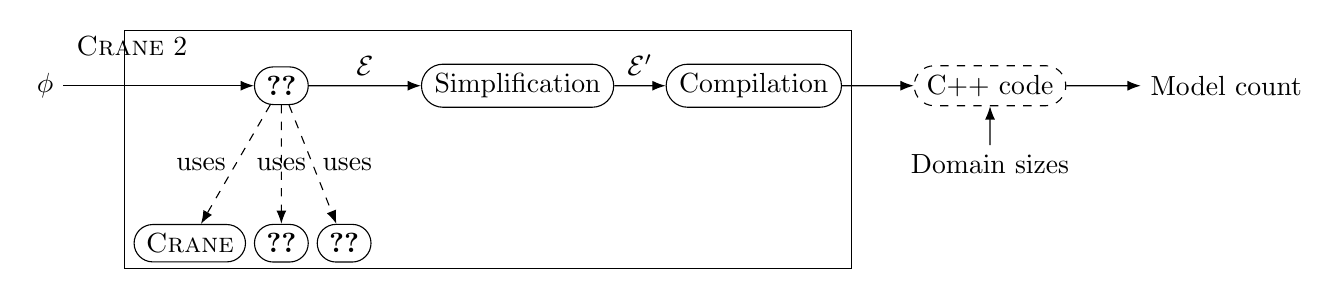
\begin{tikzpicture}
    \node at (0, 0) (formula) {$\phi$};
    \node[draw,rounded rectangle] at (3, 0) (alg1) {\Cref{alg:main}};
    \node[draw,rounded rectangle] at (6, 0) (simplification) {Simplification};
    \node[draw,rounded rectangle] at (9, 0) (compilation) {Compilation};

    \node[draw,rounded rectangle,dashed] at (12, 0) (cpp) {C++ code};
    \node at (12, -1) (sizes) {Domain sizes};

    \node at (15, 0) (count) {Model count};

    \node[draw,rounded rectangle] at (3, -2) (alg2) {\Cref{alg1}};
    \node[draw,rounded rectangle,left = 0.1cm of alg2] (crane) {\textsc{Crane}};
    \node[draw,rounded rectangle,right = 0.1cm of alg2] (alg3) {\Cref{alg2}};

    \node[draw,fit={(alg1) (simplification) (compilation) (crane) (alg2) (alg3)},inner ysep=7pt,yshift=5pt] {};
    \node at (1.1, 0.5) {\Cranetwo};

    \draw[-Latex] (formula) -- (alg1);
    \draw[-Latex] (alg1) -- node[above] {$\mathcal{E}$} (simplification);
    \draw[-Latex] (simplification) -- node[above] {$\mathcal{E}'$} (compilation);
    \draw[-Latex] (compilation) -- (cpp);
    \draw[-Latex] (sizes) -- (cpp);
    \draw[-Latex] (cpp) -- (count);

    \draw[-Latex,dashed] (alg1) -- node[midway,left] {uses} (crane);
    \draw[-Latex,dashed] (alg1) -- node[midway] {uses} (alg2);
    \draw[-Latex,dashed] (alg1) -- node[midway,right] {uses} (alg3);
  \end{tikzpicture}
  \caption{Using \Cranetwo{} to compute the model count of formula $\phi$.\ The
    formula is compiled into a set of equations $\mathcal{E}$, which are then
    algebraically simplified and compiled to a C++ program. This program can
    then be run with different command line arguments to compute the model count
    of $\phi$ for various domain sizes.}
\end{figure*}

\paragraph{Contributions (outdated).}
\begin{itemize}
  \item \Cref{sec:identifying}
  \item \Cref{sec:simplifying}
  \item Converting the recursive equations into a C++ program, which can then be
        compiled and executed to obtain numerical values (see \cref{sec:cpp}).
  \item Support for infinite precision integers using the GNU Multiple Precision
        Arithmetic Library.
  \item Some experiments vs FastWFOMC
  \item A proof of completeness
\end{itemize}

\Cref{sec:identifying,sec:cpp} deal with algebraic constructs whereas
\cref{sec:simplifying} deals with logic.

\section{Preliminaries}

\subsection{Algebra}

\paragraph{Notation.}
We write $\expr{}$ for an arbitrary algebraic expression. For any signature or
clause $C$, argument or variable $x$, and number or constant $t$, we shall write
$C[t / x]$ for the result of substituting $t$ for all occurrences of $x$ in $C$.

\begin{itemize}
  \item Variables in uppercase
  \item Domains in uppercase Greek
  \item Constant and predicate symbols in lowercase
  \item Clauses written on separate lines are implicitly conjoined
  \item For weights, for any predicate symbol $p$, we write
        $w^{+}(p), w^{-}(p) \in \mathbb{R}$ for its positive and negative
        weights, respectively. All weights not explicitly acknowledged are
        assumed to be equal to one.
\end{itemize}

\todo[inline,caption={}]{
  \begin{itemize}
    \item check if I'm still using this notation in all these cases
    \item explain how this works for function calls too
    \item introduce WFOMC as a problem
  \end{itemize}
}

\begin{definition}
  A \emph{function call} is a term of the form
  $f(x_{1} - c_{1}, \dots, x_{n} - c_{n})$ (written $f(\mathbf{x} - \mathbf{c})$
  for short), where $f$ is an $n$-ary function, each $x_{i}$ is a variable, and
  each $c_{i}$ is a non-negative constant.
\end{definition}
\todo[inline]{do I ever use this term for the case when some of the variables
  don't exist?}

\begin{definition}
  A \emph{signature} is a term of the form $f(x_{1}, \dots, x_{n})$ (written
  $f(\mathbf{x})$ for short), where $f$ is an $n$-ary function, and each $x_{i}$
  is a variable. The signature of a function call $f(\mathbf{x} - \mathbf{c})$
  is $f(\mathbf{x})$. For example, the signature of $f(x - 1, y - 2)$ is
  $f(x, y)$.
\end{definition}

\begin{definition}
  An \emph{equation} is always of the form $f(\mathbf{x}) = \expr{}$, where
  $f(\mathbf{x})$ is a signature, and $\expr{}$ is an algebraic expression.
  Henceforth, we call $f(\mathbf{x})$ and $\expr{}$ the left-hand side (LHS) and
  the right-hand side (RHS) of the equation, respectively.
\end{definition}
\todo[inline,caption={}]{
  give some examples of formulas that:
  \begin{itemize}
    \item introduce new variables,
    \item call the function itself,
    \item call some other function, and
    \item is more nested than just a sum.
  \end{itemize}
}

\begin{definition}
  A \emph{base case} is a function call where all arguments are either variables
  or constants (i.e., there is no subtraction within any argument), and there is
  at least one constant. We denote a base case in the same way as a signature,
  e.g., $f(\mathbf{x})$.
\end{definition}

\subsection{Logic}

\todo[inline,caption={}]{
  \begin{itemize}
    \item What notation am I using for FOL? Introduce equality cardinality
          constraints, counting quantifiers, etc.
    \item Need (W)FOMC semantics. What is an interpretation? What is a model?
    \item Should table caption go above or below the table?
    \item Define terms.
    \item Maybe say ``structure'' instead of interpretation?
    \item What's the right table heading capitalization for KR?
    \item Should I say ``sort'' instead of domain everywhere?
  \end{itemize}
}

\begin{table*}
  \centering
  \begin{tabular}{llclll}
    \toprule
    Logic & Sorts & Constants & Variables & Quantifiers & Additional atomic constraints\\
    \midrule
    \FO & one or more & \cmark & unlimited & $\forall$, $\exists$ & $s = t$\\
    \Ctwo & one & \xmark & two & $\forall$, $\exists$, $\exists^{= k}$, $\exists^{\le k}$, $\exists^{\ge k}$ & ---\\
    \UFO & one & \xmark & two & $\forall$ & $|p| = m$\\
    \bottomrule
  \end{tabular}
  \caption[]{A comparison of the three logics used in WFOMC in terms of:
    \begin{enumerate*}[label=(\roman*)]
      \item the number of sorts,
      \item support for constants,
      \item the maximum number of variables,
      \item allowed quantifiers, and
      \item atomic constructions in addition to those of the form $p(t_{1}, \dots, t_{n})$ for some predicate symbol $p$ and terms $t_{1}, \dots, t_{n}$.
    \end{enumerate*}
    Here:
    \begin{enumerate*}[label=(\roman*)]
      \item $k$ and $m$ are non-negative integers, the latter of which can depend on the domain size,
      \item $p$ is a predicate symbol, and
      \item $s$ and $t$ are terms.
    \end{enumerate*}
  }\label{tbl:logics}
\end{table*}

\paragraph{Three types of logics}
\begin{itemize}
  \item All three logics are function-free.
  \item Domains are always assumed to be finite.
  \item See \cref{tbl:logics} for a detailed comparison. \FO{} is used as the
        input format for \textsc{ForcLift} and its extensions \textsc{Crane} and
        \Cranetwo{}. \Ctwo{} is used in the literature on \textsc{FastWFOMC} and
        related methods (TODO: citations). \UFO{} is the input format supported
        by a privately-obtained version of \textsc{FastWFOMC}. Note that the
        publicly available version does not support any cardinality constraints.
  \item In the case of \textsc{ForcLift} and its extensions, support for a
        formula as valid input does not imply that the algorithm will be able to
        compile the formula into a circuit or graph suitable for lifted model
        counting. However, it is known that \textsc{ForcLift} compilation is
        guaranteed to succeed on any \FO{} formula without constants and with at
        most two variables (TODO: citation).
\end{itemize}

A \emph{formula} is a set of clauses. A \emph{clause} is of the form
$\forall x_{1} \in \Delta_{1}\forall x_{2} \in \Delta_{2}\dots\forall x_{n} \in \Delta_{n} \phi(x_{1}, x_{2}, \dots, x_{n})$,
where $\phi$ is a disjunction of literals that only contain variables
$x_{1}, \dots, x_{n}$ (and any constants). A \emph{literal} is either an atom or
its negation. An \emph{atom} is of the form $P(t_{1}, \dots, t_{m})$, where $P$
is a predicate, and $t_{1}, \dots, t_{m}$ are terms. A \emph{term} is either a
variable or a constant.

\todo[inline]{explain set-based notation for a clause (iterating over all
  literals)}

For any clause or literal $l$, let $\Vars(l)$ denote the set of variables in
$l$.

For any (bound) variable $v$, let $\Dom(v)$ denote the domain over which $v$ is
quantified. For a literal $l$,
$\Doms(l) \coloneqq \{\, \Dom(v) \mid v \in \Vars(l) \,\}$. Similarly, for any
clause $C$, let $\Doms(C) = \{\, \Dom(v) \mid v \in \Vars(C) \,\}$.

\section{Completing the Definitions of Recursive Functions}\label{sec:main}

\begin{algorithm}[t]
  \caption{The core part of \Cranetwo{} that compiles a formula...}\label{alg:main}% TODO: start here
  \KwIn{formula $\phi$}
  \KwOut{set $\mathcal{E}$ of equations}
  $(\mathcal{E}, \mathcal{F}, \mathcal{D}) \gets \Crane{$\phi$}$\;
  \ForEach{base case $f(\mathbf{x}) \in \FindBaseCases{$\mathcal{E}$}$}{
    $\psi \gets \mathcal{F}(f)$\;
    \ForEach{$i$ such that $x_{i}$ is a constant}{
      $\psi \gets \Propagate{$\psi$, $\mathcal{D}(f, i)$, $x_i$}$\;
    }
    $(\mathcal{E}', \text{\textunderscore}, \text{\textunderscore}) \gets \Crane{$\psi$}$\;
    $\mathcal{E} \gets \mathcal{E} \cup \mathcal{E}'$\;
  }
\end{algorithm}

See \cref{alg:main}.

We write \Crane for a slight modification of the original \textsc{Crane} that
compiles a formula $\phi$ into:
\begin{itemize}
  \item a set $\mathcal{E}$ of equations,
  \item a map $\mathcal{F}$ from function names to formulas, and
  \item a map $\mathcal{D}$ from function names and parameter indices to
        domains.
\end{itemize}

% TODO: update: crane or crane2
The evaluation of base cases is done by simplifying the clauses and then using
\textsc{Crane} to find the base cases. A particular domain is selected, and the
clauses are simplified. Then, \textsc{Crane} is called on those clauses to
evaluate the base cases. After that, we change the function names and variable
to make it consistent with the previous domain to variable mapping, and append
these base cases to the set of equations.

\todo[inline,caption={}]{extend it to work with base cases that are themselves
  recursive}

\subsection{Identifying a Sufficient Set of Base Cases}\label{sec:identifying}

\begin{algorithm}[t]
  \caption{\protect\FindBaseCases{$\mathcal{E}$}}\label{alg1}
  \KwIn{set $\mathcal{E}$ of equations}
  \KwOut{set $\mathcal{B}$ of base cases}

  $\mathcal{B} \gets \emptyset$\;
  \ForEach{equation $(f(\mathbf{x}) = \expr{}) \in \mathcal{E}$}{
    \ForEach{function call $f(\mathbf{x} - \mathbf{c}) \in \expr{}$}{\label{line:functioncall}
      \ForEach{$c_{i} \in \mathbf{c}$}{
        \For{$n \gets 0$ \KwTo $c_{i} - 1$}{\label{line:lim}
          $\mathcal{B} \gets \mathcal{B} \cup \{\, f(\mathbf{x})[x_{i}/n] \,\}$\;\label{line:insert}
        }
      }
    }
  }
\end{algorithm}

The algorithm is described as \cref{alg1}. We know that if, say, on the RHS of
all equations, the domain size appears as $m - c_1, m - c_2, \dots, m - c_k$,
then finding $f(0, x_1, x_2, \dots)$, $f(1, x_1, x_2, \dots)$,
$\dots f(m_0, x_1, x_2, \dots)$ for every function $f$, where
$m_0 = \max(c_1, c_2, \dots c_k) - 1$ forms a sufficient set of base cases.
Hence, in order to do the same efficiently, we can take that domain for which
$m_0$ is the minimum, i.e. $\argmin(\max(c_1, c_2, \dots c_k))$. Ideally, we
should calculate the base cases by finding the base cases up to
$\max(c_{1}, c_{2}, \dots) - 1$. However, currently only empty and singleton
domains are supported.

First, expand the summations in each equation. Here we expand the summations of
the form: $\sum_{x=0}^{x_{1}} \expr{} \cdot [a \le x < b]$ or similar
inequalities where $x$ is bounded by constants and $a$ and $b$ are constants, by
substituting the value of $x$ from $a$ to $b-1$. For example, we replace
$\sum_{x=0}^{x_1} \binom{x_{1}}{x} f(x_1 - x) \cdot [0 \le x < 2]$ by
$\binom{x_{1}}{0} f(x_1) + \binom{x_{1}}{1} f(x_1-1)$.

\begin{itemize}
  \item \cref{line:insert} for $f(\mathbf{x}) = f(y, z)$, $x_{i} = y$, and
        $n = 0$, add $f(y, z)[y/0] = f(0, z)$ to $\mathcal{B}$.
\end{itemize}

\begin{theorem}
  Under the following assumptions, \cref{alg1} is guaranteed to return a
  sufficient set of base cases:
  \begin{itemize}
    \item there is no mutual recursion
    \item each function $f$ has exactly one equation with $f$ on the LHS;
    \item in the recursive definition of function $f(x_{1},\dots,x_{n})$, the
          $i$-th argument of each call to $f$ on the RHS is of the form
          $x_{i} - c_{i}$, where:
          \begin{itemize}
            \item $c_{i} \ge 0$ for all $i$, and
            \item $c_{i} > 0$ for at least one $i$.
          \end{itemize}
  \end{itemize}
\end{theorem}

\begin{example}
  For an equation $f(m, n) = 2 \times f(m-1, n)$, \cref{alg1} returns $f(0, n)$.
\end{example}

NOTE: function calls such as $f(n-m)$ and $f(n-m-1)$ are ignored.

\subsection{Propagating Domain Size Assumptions}\label{sec:simplifying}

\begin{algorithm}[t]
  \caption{\protect\Propagate{$\phi$, $\Delta$, $n$} TODO: find the source code and check: (1) what we're doing with unit clauses, (2) whether we just randomly pick any literal to negate}\label{alg2}
  \KwIn{formula $\phi$, domain $\Delta$, domain size $n \in \{\, 0, 1 \,\}$}
  \KwOut{formula $\phi'$}
  $\phi' \gets \emptyset$\;
  \uIf{$n = 0$}{
    \ForEach{clause $C \in \phi$}{
      \lIf{$\Delta \not\in \Doms(C)$}{$\phi' \gets \phi' \cup \{\, C \,\}$}
      $C' \gets \{\, l \in C \mid \Delta \not\in \Doms(l) \,\}$\;
      \If{$\Delta \in \Doms(C)$ {\bf and} $C' \ne \emptyset$}{
        $l \gets \text{an arbitrary literal in } C'$\;\label{line:smoothing1}
        $\phi' \gets \phi' \cup \{\, C' \cup \{\, \neg l \,\} \,\} $\;\label{line:smoothing2}
      }
    }
  }
  \Else{
    $c \gets$ a new constant symbol\;
    \ForEach{clause $C \in \phi$}{
      $C' \gets C$\;
      \ForEach{$v \in \Vars(C)$ with $\Dom(v) = \Delta$}{
        $C' \gets C'[c / v]$\;
      }
      $\phi' \gets \phi' \cup \{\, C' \,\}$\;
    }
  }
\end{algorithm}

We use \cref{alg2} to find the transformed formula corresponding to each base
case obtained using \cref{alg1} and call \textsc{Crane} on the formula to obtain
the required base cases.
% TODO: or crane 2?

\begin{itemize}
  \item Clauses where all literals have variables quantified over the empty
        domain are still removed.
  \item $C'$ is guaranteed to be non-empty.
  \item \Cref{line:smoothing1,line:smoothing2} are explained in
        \cref{sec:smoothingbase}.
\end{itemize}

\section{Smoothing}

Goal of smoothing: whenever rules such as unit propagation or
inclusion-exclusion (maybe just these two?) eliminate the consideration of some
ground atoms, smoothing nodes should be inserted `at the same level' so that
these ground atoms are still considered when counting. Note that conjunction
nodes are irrelevant here because multiplication is associative. `At the same
level' means that, e.g., if some ground atoms were eliminated from consideration
before/after performing independent partial grounding, then the smoothing node
should also appear before/after the independent partial grounding node.

\todo[inline,caption={}]{
  \begin{itemize}
    \item Can I prove that the additions to smoothing outlined in the rest of
          this section `do the right thing'?
    \item I could include more info about the smoothing algorithm that didn't
          make it into the previous paper.
  \end{itemize}
}

\subsection{Smoothing for Base Cases}\label{sec:smoothingbase}

\paragraph{Key point.}
If there is a predicate $p$ that has nothing to do with domain $\Delta$, make
sure that $p$ remains as part of the formula even if all clauses with $p$ can be
removed. Which literal is picked on \cref{line:smoothing1} of \cref{alg2} is not
important because any choice achieves the same goal: constructing a clause that
mentions the same predicates as $C'$ and is satisfied by any interpretation.

\begin{fact}
  Assuming that domain $\Delta$ is empty, any clause that contains
  `$\forall x \in \Delta$' (for any variable $x$) is vacuously satisfied by all
  interpretations.
\end{fact}

For example, consider the formula
\begin{align}
  \forall x \in \Delta \forall y, z \in \Gamma &: P(x) \lor Q(y, z)\label[formula]{eq:example1}\\
  \forall y, z \in \Gamma' &: Q(y, z)\label[formula]{eq:example2}
\end{align}
and assume that $\Gamma' \subseteq \Gamma$. In this case, if we set $|\Delta|$
to zero and remove clauses with variables quantified over $\Delta$, we get
\begin{equation}\label[formula]{eq:simplified}
  \forall y, z \in \Gamma' : Q(y, z),
\end{equation}
but the model count of \cref{eq:simplified} is one. However, the actual model
count should be $2^{|\Gamma|^2 - |\Gamma'|^2}$. That is, $Q$ as a relation is a
subset of $\Gamma \times \Gamma$. While \cref{eq:example1} becomes vacuously
true, \cref{eq:example2} fixes the value of $Q$ over
$\Gamma' \times \Gamma' \subseteq \Gamma \times \Gamma$. Hence, the number of
different values that $Q$ can take is
$|(\Gamma \times \Gamma) \setminus (\Gamma' \times \Gamma')| = |\Gamma|^{2} - |\Gamma'|^{2}$.

We address this issue by converting clauses with universal quantifiers over the
empty domain to tautologies, hence retaining all the predicates that have no
argument assigned to the empty domain. For example, we would convert
\cref{eq:example1,eq:example2} to
\begin{align*}
  \forall y, z \in \Gamma &: Q(y, z) \lor \neg Q(y, z) \\
  \forall y, z \in \Gamma' &: Q(y, z).
\end{align*}
The model count returned by this will also consider the truth value of $Q$ over
$y \in \Gamma \setminus \Gamma'$ or $z \in \Gamma \setminus \Gamma'$.

\subsection{Stage 1: Propagating Unit Clauses `Upwards'}

\begin{description}
  \item[\texttt{Ref}.] During smoothing, when unit clauses (a.k.a.\ variables)
        are propagated in the opposite direction of the FCG arcs (i.e.,
        `upwards'), when visiting a \texttt{Ref} node, these clauses are
        translated using the domain map of the \texttt{Ref} node. For example,
        if the domain map include $\Delta \mapsto \Delta'$, and the unit clause
        mentions $\Delta$, then replace it by $\Delta'$.
  \item[Constraint removal.] Do reverse constraint removal. Assuming that
        domain $\Delta$ with constraints $X \ne c$ (for some constant
        $c \in \Delta$) were replaced with domain $\Delta'$, replace each
        $\forall X \in \Delta'\text{. }\phi(X)$ with
        $\forall X \in \Delta\text{. }X \ne c \Rightarrow \phi(X)$.
  \item[Domain recursion.] Suppose the domain recursion node introduces constant
        $x \in \Delta$. For each unit clause received from the child node,
        replace each occurrence of $\phi(x)$ or $\forall X \in \Delta\text{.
        } X \ne x \Rightarrow \phi(X)$ with $\forall X \in \Delta\text{.
        }\phi(X)$. This can be seen as a claim about what ground atoms the
        domain recursion node \emph{should} cover (or a temporary assumption).
        If the relevant subgraph indeed covers those ground atoms, Stage~2 will
        do nothing. Otherwise, smoothing nodes will be added below the domain
        recursion node to cover the difference between what was propagated from
        the domain recursion node and what was received from the child node.
\end{description}
\todo[inline]{Add examples of both cases, with figures.}

\subsection{Stage 2: Adding Smoothing Nodes}

% TODO
% \item Whenever the set of unit clauses received from the child node contains two
% formulas $\phi(x)$ and $\forall X \in \Delta\text{.
% } X \ne x \Rightarrow \phi(X)$ (i.e., the only difference between the two
% formulas is that one has the constant $x$ whereas the other one has a variable
% $X \ne x$), merge them into $\forall X \in \Delta\text{. }\phi(X)$.

\begin{description}
  \item[\texttt{Ref}:] nothing.
  \item[Constraint removal:] nothing.
  \item[Domain recursion:]
        \begin{enumerate}
          \item Whenever the set of unit clauses of the child node contains two
                formulas $\phi(x)$ and $\forall X \in \Delta\text{.
                } X \ne x \Rightarrow \phi(X)$ (i.e., the only difference
                between the two formulas is that one has the constant $x$
                whereas the other one has a variable $X \ne x$), merge them into
                $\forall X \in \Delta\text{. }\phi(X)$.
          \item Add smoothing nodes below the domain recursion node for the
                difference between the unit clauses assigned to the domain
                recursion node during Stage 1 and the unit clauses of the child
                node post-processed by the step above. For example, if the child
                node `covers' only $p(x)$, then Stage 1 assigns
                $\forall X \in \Delta\text{. }p(X)$ to the domain recursion
                node. The smoothing node below the domain recursion node then
                has the clause $\forall X \in \Delta\text{.
                } X \ne x \Rightarrow p(X)$.
        \end{enumerate}
\end{description}

\todo[inline]{Can I formally define what is meant by `difference'?}

\section{Generating C++ Code}\label{sec:cpp}

The target is to generate C++ code that can evaluate numerical values of the
model counts based on the equations generated by \textsc{Crane}. We achieve this
by parsing the equations generated by \textsc{Crane}, simplifying them, and then
generating C++ code. This approach can be done in linear time in the length of
the formula using
the
\href{https://en.wikipedia.org/wiki/Shunting_yard_algorithm#:~:text=In%20computer%20science%2C%20the%20shunting,abstract%20syntax%20tree%20(AST).}{Shunting
  Yard Algorithm}.

The translation of a set $\mathcal{E}$ of equations into a C++ program works as
follows.

First, we create a cache for each function in $\mathcal{E}$. This is implemented
as a multi-dimensional vector containing objects of \texttt{class cache\_elem}
defined as shown in the example code. The default initialization of this object
is to $-1$ which is useful for recognizing unevaluated cases.

Next, we create a function definition for the LHS of each equation in
$\mathcal{E}$, including all functions and base cases. The signatures of these
functions is decided as follows. A function call containing only variable
arguments is named as the function itself, and ones with constants in their
arguments are suffixed with a string that contains \texttt{'x'} at the $i$th
place if the $i$th argument is variable and the $i$th argument if that argument
is a constant. For example, $f(x_{1}, x_{2}, x_{3})$ is declared as \texttt{int
  f(int x1, int x2, int x3);} and $f(1, x_{2}, x_{3})$ is declared as
\texttt{int f\_1xx(int x2, int x3);} (the constant arguments are removed from
the signature).

The RHS of each equation in $\mathcal{E}$ is used to define the body of the
equation corresponding to the LHS of that equation. The function body (for a
function \texttt{func} corresponding to equation $e$) is formed as follows.

First, we check if the evaluation is already present in the cache. If so, then
we return the cache element. The cache accesses are done using the
\texttt{get\_elem} function (definition given in the example), which resizes the
cache if the accessed index is out of range.

Second, if the element is absent, then we decide if the arguments corresponding
to $e$ or one of the functions corresponding to the base cases, based on the
value of the arguments. If it corresponds to the base cases, then we directly
call the base case function and return its value. Else, we evaluate the value
using the RHS, store the evaluated value in the cache and return the evaluated
value. Note that in this step, we only call the base case function with one more
constant argument than \texttt{func}. For example, \texttt{f0(x, y)} would call
\texttt{f0\_0x(y)} if $x = 0$ and \texttt{f0\_x0(x)} if $y = 0$.

Third, to translate the RHS, we convert $\sum_{x=a}^{b} \expr{}$ to
\begin{lstlisting}[escapeinside={(*}{*)}]
([y,z,...](){
    int sum = 0;
    for(int x = a; x <= b; x++)
        sum += (*$\expr{}$*);
    return sum;
})()
\end{lstlisting}
where $y, z, \dots$ are the free variables present in $\expr{}$.

\section{Experiments}

Comparing \textsc{Crane} and \textsc{FastWFOMC} on a larger set of benchmarks is
challenging because there is no automated way to translate a formula in \FO{} or
\Ctwo{} into \UFO{} (or even check if such an encoding is possible).

\paragraph{Benchmarks (probably for supplementary material).}
\begin{itemize}
  \item Functions
        \begin{itemize}
          \item In \Ctwo: $\forall X \in \Delta\text{.
                }\exists^{=1} Y \in \Delta\text{. }p(X, Y)$
          \item In \UFO:
                \begin{gather*}
                  \forall X, Y \in \Delta\text{. } s(X) \lor \neg p(X, Y)\\
                  |p| = |\Delta|
                \end{gather*}
          \item In \FO:
                \begin{gather*}
                  \forall X \in \Delta\text{. }\exists Y \in \Delta\text{. } p(X, Y)\\
                  \forall X, Y, Z \in \Delta\text{. } p(X, Y) \land p(X, Z) \Rightarrow Y = Z
                \end{gather*}
        \end{itemize}
  \item Permutations
        \begin{itemize}
          \item In \Ctwo:
                \begin{gather*}
                  \forall X \in \Delta\text{. }\exists^{=1} Y \in \Delta\text{. }p(X, Y)\\
                  \forall Y \in \Delta\text{. }\exists^{=1} X \in \Delta\text{. }p(X, Y)
                \end{gather*}
          \item In \UFO:
                \begin{gather*}
                  \forall X, Y \in \Delta\text{. } r(X) \lor \neg p(X, Y)\\
                  \forall X, Y \in \Delta\text{. } s(X) \lor \neg p(Y, X)\\
                  |p| = |\Delta|
                \end{gather*}
                with weights $w^{-}(r) = w^{-}(s) = -1$
          \item In \FO:
                \begin{gather*}
                  \forall X \in \Delta\text{. }\exists Y \in \Delta\text{. } p(X, Y)\\
                  \forall Y \in \Delta\text{. }\exists X \in \Delta\text{. } p(X, Y)\\
                  \forall X, Y, Z \in \Delta\text{. } p(X, Y) \land p(X, Z) \Rightarrow Y = Z\\
                  \forall X, Y, Z \in \Delta\text{. } p(X, Y) \land p(Z, Y) \Rightarrow X = Z
                \end{gather*}
        \end{itemize}
\end{itemize}

\paragraph{Setup.}
\begin{itemize}
  \item The experiments were run on an AMD~Ryzen~7~5800H processor with
        \SI{16}{\gibi\byte} of memory and Arch Linux~6.8.2-arch2-1 operating
        system. \textsc{FastWFOMC} was run using Python~3.8.19 with
        Python-FLINT~0.5.0.
\end{itemize}

\begin{figure}
  \centering
  % Created by tikzDevice version 0.12.6 on 2024-08-15 12:12:55
% !TEX encoding = UTF-8 Unicode
\documentclass[10pt]{article}
\usepackage{tikz}

\usepackage[active,tightpage,psfixbb]{preview}

\PreviewEnvironment{pgfpicture}

\setlength\PreviewBorder{0pt}
\begin{document}

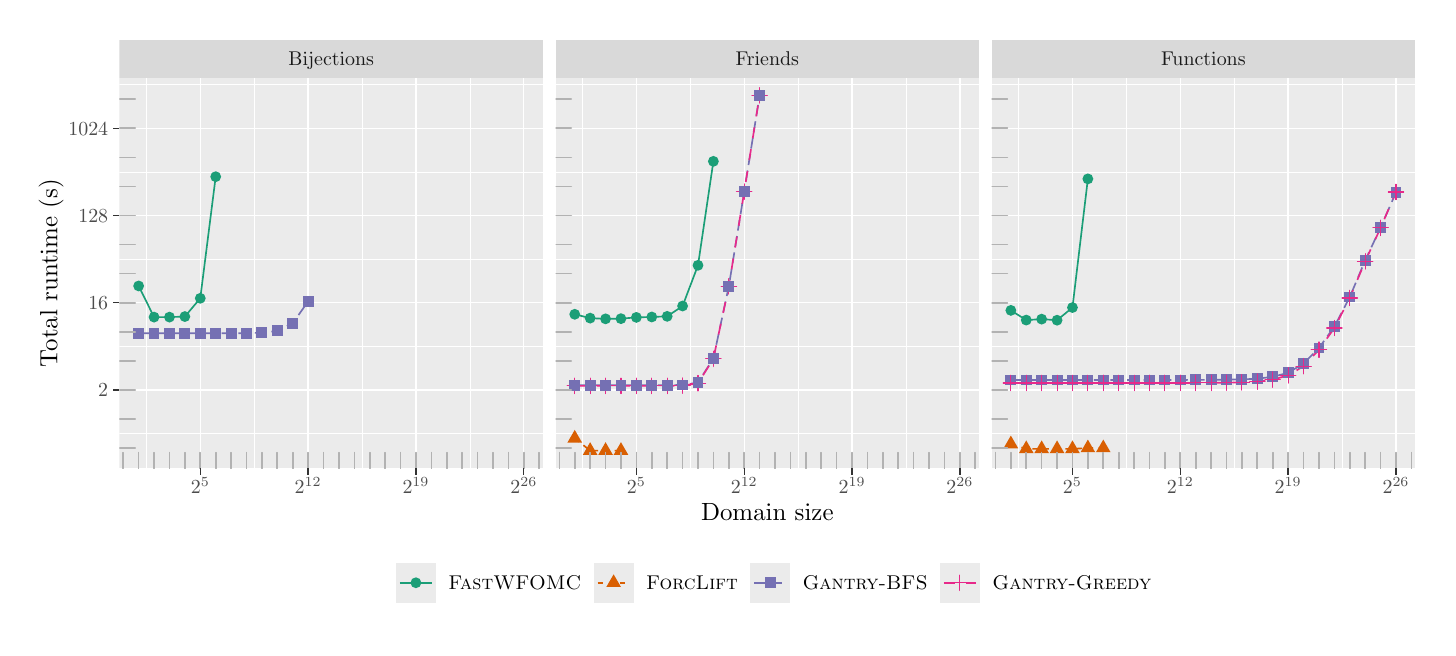
\begin{tikzpicture}[x=1pt,y=1pt]
\definecolor{fillColor}{RGB}{255,255,255}
\path[use as bounding box,fill=fillColor,fill opacity=0.00] (0,0) rectangle (505.89,216.81);
\begin{scope}
\path[clip] (  0.00,  0.00) rectangle (505.89,216.81);
\definecolor{drawColor}{RGB}{255,255,255}
\definecolor{fillColor}{RGB}{255,255,255}

\path[draw=drawColor,line width= 0.5pt,line join=round,line cap=round,fill=fillColor] ( -0.00,  0.00) rectangle (505.89,216.81);
\end{scope}
\begin{scope}
\path[clip] ( 33.14, 57.56) rectangle (186.23,198.75);
\definecolor{fillColor}{gray}{0.92}

\path[fill=fillColor] ( 33.14, 57.56) rectangle (186.23,198.75);
\definecolor{drawColor}{RGB}{255,255,255}

\path[draw=drawColor,line width= 0.2pt,line join=round] ( 33.14, 70.17) --
	(186.23, 70.17);

\path[draw=drawColor,line width= 0.2pt,line join=round] ( 33.14,101.68) --
	(186.23,101.68);

\path[draw=drawColor,line width= 0.2pt,line join=round] ( 33.14,133.19) --
	(186.23,133.19);

\path[draw=drawColor,line width= 0.2pt,line join=round] ( 33.14,164.70) --
	(186.23,164.70);

\path[draw=drawColor,line width= 0.2pt,line join=round] ( 33.14,196.21) --
	(186.23,196.21);

\path[draw=drawColor,line width= 0.2pt,line join=round] ( 42.89, 57.56) --
	( 42.89,198.75);

\path[draw=drawColor,line width= 0.2pt,line join=round] ( 81.85, 57.56) --
	( 81.85,198.75);

\path[draw=drawColor,line width= 0.2pt,line join=round] (120.82, 57.56) --
	(120.82,198.75);

\path[draw=drawColor,line width= 0.2pt,line join=round] (159.78, 57.56) --
	(159.78,198.75);

\path[draw=drawColor,line width= 0.5pt,line join=round] ( 33.14, 85.92) --
	(186.23, 85.92);

\path[draw=drawColor,line width= 0.5pt,line join=round] ( 33.14,117.43) --
	(186.23,117.43);

\path[draw=drawColor,line width= 0.5pt,line join=round] ( 33.14,148.95) --
	(186.23,148.95);

\path[draw=drawColor,line width= 0.5pt,line join=round] ( 33.14,180.46) --
	(186.23,180.46);

\path[draw=drawColor,line width= 0.5pt,line join=round] ( 62.37, 57.56) --
	( 62.37,198.75);

\path[draw=drawColor,line width= 0.5pt,line join=round] (101.34, 57.56) --
	(101.34,198.75);

\path[draw=drawColor,line width= 0.5pt,line join=round] (140.30, 57.56) --
	(140.30,198.75);

\path[draw=drawColor,line width= 0.5pt,line join=round] (179.27, 57.56) --
	(179.27,198.75);
\definecolor{drawColor}{RGB}{27,158,119}

\path[draw=drawColor,line width= 0.6pt,line join=round] ( 40.10,123.48) --
	( 45.67,112.22) --
	( 51.24,112.22) --
	( 56.80,112.42) --
	( 62.37,119.02) --
	( 67.94,162.96);
\definecolor{drawColor}{RGB}{117,112,179}

\path[draw=drawColor,line width= 0.6pt,dash pattern=on 4pt off 2pt ,line join=round] ( 40.10,106.36) --
	( 45.67,106.36) --
	( 51.24,106.36) --
	( 56.80,106.36) --
	( 62.37,106.36) --
	( 67.94,106.37) --
	( 73.50,106.38) --
	( 79.07,106.42) --
	( 84.64,106.58) --
	( 90.20,107.23) --
	( 95.77,109.99) --
	(101.34,117.90);
\definecolor{fillColor}{RGB}{117,112,179}

\path[fill=fillColor] ( 38.14,104.40) --
	( 42.06,104.40) --
	( 42.06,108.33) --
	( 38.14,108.33) --
	cycle;

\path[fill=fillColor] ( 43.71,104.40) --
	( 47.63,104.40) --
	( 47.63,108.33) --
	( 43.71,108.33) --
	cycle;

\path[fill=fillColor] ( 49.27,104.40) --
	( 53.20,104.40) --
	( 53.20,108.33) --
	( 49.27,108.33) --
	cycle;

\path[fill=fillColor] ( 54.84,104.40) --
	( 58.76,104.40) --
	( 58.76,108.33) --
	( 54.84,108.33) --
	cycle;

\path[fill=fillColor] ( 60.41,104.40) --
	( 64.33,104.40) --
	( 64.33,108.33) --
	( 60.41,108.33) --
	cycle;

\path[fill=fillColor] ( 65.97,104.40) --
	( 69.90,104.40) --
	( 69.90,108.33) --
	( 65.97,108.33) --
	cycle;

\path[fill=fillColor] ( 71.54,104.41) --
	( 75.46,104.41) --
	( 75.46,108.34) --
	( 71.54,108.34) --
	cycle;

\path[fill=fillColor] ( 77.11,104.45) --
	( 81.03,104.45) --
	( 81.03,108.38) --
	( 77.11,108.38) --
	cycle;

\path[fill=fillColor] ( 82.67,104.62) --
	( 86.60,104.62) --
	( 86.60,108.54) --
	( 82.67,108.54) --
	cycle;

\path[fill=fillColor] ( 88.24,105.27) --
	( 92.16,105.27) --
	( 92.16,109.19) --
	( 88.24,109.19) --
	cycle;

\path[fill=fillColor] ( 93.81,108.02) --
	( 97.73,108.02) --
	( 97.73,111.95) --
	( 93.81,111.95) --
	cycle;

\path[fill=fillColor] ( 99.37,115.94) --
	(103.30,115.94) --
	(103.30,119.87) --
	( 99.37,119.87) --
	cycle;
\definecolor{fillColor}{RGB}{27,158,119}

\path[fill=fillColor] ( 40.10,123.48) circle (  1.96);

\path[fill=fillColor] ( 45.67,112.22) circle (  1.96);

\path[fill=fillColor] ( 51.24,112.22) circle (  1.96);

\path[fill=fillColor] ( 56.80,112.42) circle (  1.96);

\path[fill=fillColor] ( 62.37,119.02) circle (  1.96);

\path[fill=fillColor] ( 67.94,162.96) circle (  1.96);
\definecolor{drawColor}{gray}{0.70}

\path[draw=drawColor,line width= 0.6pt,line join=round,line cap=round] ( 34.54, 57.56) -- ( 34.54, 63.25);

\path[draw=drawColor,line width= 0.6pt,line join=round,line cap=round] ( 40.10, 57.56) -- ( 40.10, 63.25);

\path[draw=drawColor,line width= 0.6pt,line join=round,line cap=round] ( 45.67, 57.56) -- ( 45.67, 63.25);

\path[draw=drawColor,line width= 0.6pt,line join=round,line cap=round] ( 51.24, 57.56) -- ( 51.24, 63.25);

\path[draw=drawColor,line width= 0.6pt,line join=round,line cap=round] ( 56.80, 57.56) -- ( 56.80, 63.25);

\path[draw=drawColor,line width= 0.6pt,line join=round,line cap=round] ( 62.37, 57.56) -- ( 62.37, 63.25);

\path[draw=drawColor,line width= 0.6pt,line join=round,line cap=round] ( 67.94, 57.56) -- ( 67.94, 63.25);

\path[draw=drawColor,line width= 0.6pt,line join=round,line cap=round] ( 73.50, 57.56) -- ( 73.50, 63.25);

\path[draw=drawColor,line width= 0.6pt,line join=round,line cap=round] ( 79.07, 57.56) -- ( 79.07, 63.25);

\path[draw=drawColor,line width= 0.6pt,line join=round,line cap=round] ( 84.64, 57.56) -- ( 84.64, 63.25);

\path[draw=drawColor,line width= 0.6pt,line join=round,line cap=round] ( 90.20, 57.56) -- ( 90.20, 63.25);

\path[draw=drawColor,line width= 0.6pt,line join=round,line cap=round] ( 95.77, 57.56) -- ( 95.77, 63.25);

\path[draw=drawColor,line width= 0.6pt,line join=round,line cap=round] (101.34, 57.56) -- (101.34, 63.25);

\path[draw=drawColor,line width= 0.6pt,line join=round,line cap=round] (106.90, 57.56) -- (106.90, 63.25);

\path[draw=drawColor,line width= 0.6pt,line join=round,line cap=round] (112.47, 57.56) -- (112.47, 63.25);

\path[draw=drawColor,line width= 0.6pt,line join=round,line cap=round] (118.04, 57.56) -- (118.04, 63.25);

\path[draw=drawColor,line width= 0.6pt,line join=round,line cap=round] (123.60, 57.56) -- (123.60, 63.25);

\path[draw=drawColor,line width= 0.6pt,line join=round,line cap=round] (129.17, 57.56) -- (129.17, 63.25);

\path[draw=drawColor,line width= 0.6pt,line join=round,line cap=round] (134.74, 57.56) -- (134.74, 63.25);

\path[draw=drawColor,line width= 0.6pt,line join=round,line cap=round] (140.30, 57.56) -- (140.30, 63.25);

\path[draw=drawColor,line width= 0.6pt,line join=round,line cap=round] (145.87, 57.56) -- (145.87, 63.25);

\path[draw=drawColor,line width= 0.6pt,line join=round,line cap=round] (151.44, 57.56) -- (151.44, 63.25);

\path[draw=drawColor,line width= 0.6pt,line join=round,line cap=round] (157.00, 57.56) -- (157.00, 63.25);

\path[draw=drawColor,line width= 0.6pt,line join=round,line cap=round] (162.57, 57.56) -- (162.57, 63.25);

\path[draw=drawColor,line width= 0.6pt,line join=round,line cap=round] (168.13, 57.56) -- (168.13, 63.25);

\path[draw=drawColor,line width= 0.6pt,line join=round,line cap=round] (173.70, 57.56) -- (173.70, 63.25);

\path[draw=drawColor,line width= 0.6pt,line join=round,line cap=round] (179.27, 57.56) -- (179.27, 63.25);

\path[draw=drawColor,line width= 0.6pt,line join=round,line cap=round] (184.83, 57.56) -- (184.83, 63.25);

\path[draw=drawColor,line width= 0.6pt,line join=round,line cap=round] ( 33.14, 64.92) -- ( 38.84, 64.92);

\path[draw=drawColor,line width= 0.6pt,line join=round,line cap=round] ( 33.14, 75.42) -- ( 38.84, 75.42);

\path[draw=drawColor,line width= 0.6pt,line join=round,line cap=round] ( 33.14, 85.92) -- ( 38.84, 85.92);

\path[draw=drawColor,line width= 0.6pt,line join=round,line cap=round] ( 33.14, 96.43) -- ( 38.84, 96.43);

\path[draw=drawColor,line width= 0.6pt,line join=round,line cap=round] ( 33.14,106.93) -- ( 38.84,106.93);

\path[draw=drawColor,line width= 0.6pt,line join=round,line cap=round] ( 33.14,117.43) -- ( 38.84,117.43);

\path[draw=drawColor,line width= 0.6pt,line join=round,line cap=round] ( 33.14,127.94) -- ( 38.84,127.94);

\path[draw=drawColor,line width= 0.6pt,line join=round,line cap=round] ( 33.14,138.44) -- ( 38.84,138.44);

\path[draw=drawColor,line width= 0.6pt,line join=round,line cap=round] ( 33.14,148.95) -- ( 38.84,148.95);

\path[draw=drawColor,line width= 0.6pt,line join=round,line cap=round] ( 33.14,159.45) -- ( 38.84,159.45);

\path[draw=drawColor,line width= 0.6pt,line join=round,line cap=round] ( 33.14,169.95) -- ( 38.84,169.95);

\path[draw=drawColor,line width= 0.6pt,line join=round,line cap=round] ( 33.14,180.46) -- ( 38.84,180.46);

\path[draw=drawColor,line width= 0.6pt,line join=round,line cap=round] ( 33.14,190.96) -- ( 38.84,190.96);
\end{scope}
\begin{scope}
\path[clip] (190.73, 57.56) rectangle (343.81,198.75);
\definecolor{fillColor}{gray}{0.92}

\path[fill=fillColor] (190.73, 57.56) rectangle (343.81,198.75);
\definecolor{drawColor}{RGB}{255,255,255}

\path[draw=drawColor,line width= 0.2pt,line join=round] (190.73, 70.17) --
	(343.81, 70.17);

\path[draw=drawColor,line width= 0.2pt,line join=round] (190.73,101.68) --
	(343.81,101.68);

\path[draw=drawColor,line width= 0.2pt,line join=round] (190.73,133.19) --
	(343.81,133.19);

\path[draw=drawColor,line width= 0.2pt,line join=round] (190.73,164.70) --
	(343.81,164.70);

\path[draw=drawColor,line width= 0.2pt,line join=round] (190.73,196.21) --
	(343.81,196.21);

\path[draw=drawColor,line width= 0.2pt,line join=round] (200.47, 57.56) --
	(200.47,198.75);

\path[draw=drawColor,line width= 0.2pt,line join=round] (239.43, 57.56) --
	(239.43,198.75);

\path[draw=drawColor,line width= 0.2pt,line join=round] (278.40, 57.56) --
	(278.40,198.75);

\path[draw=drawColor,line width= 0.2pt,line join=round] (317.37, 57.56) --
	(317.37,198.75);

\path[draw=drawColor,line width= 0.5pt,line join=round] (190.73, 85.92) --
	(343.81, 85.92);

\path[draw=drawColor,line width= 0.5pt,line join=round] (190.73,117.43) --
	(343.81,117.43);

\path[draw=drawColor,line width= 0.5pt,line join=round] (190.73,148.95) --
	(343.81,148.95);

\path[draw=drawColor,line width= 0.5pt,line join=round] (190.73,180.46) --
	(343.81,180.46);

\path[draw=drawColor,line width= 0.5pt,line join=round] (219.95, 57.56) --
	(219.95,198.75);

\path[draw=drawColor,line width= 0.5pt,line join=round] (258.92, 57.56) --
	(258.92,198.75);

\path[draw=drawColor,line width= 0.5pt,line join=round] (297.88, 57.56) --
	(297.88,198.75);

\path[draw=drawColor,line width= 0.5pt,line join=round] (336.85, 57.56) --
	(336.85,198.75);
\definecolor{drawColor}{RGB}{27,158,119}

\path[draw=drawColor,line width= 0.6pt,line join=round] (197.68,113.24) --
	(203.25,111.85) --
	(208.82,111.59) --
	(214.38,111.66) --
	(219.95,112.12) --
	(225.52,112.27) --
	(231.08,112.50) --
	(236.65,116.23) --
	(242.22,130.94) --
	(247.78,168.51);
\definecolor{drawColor}{RGB}{217,95,2}

\path[draw=drawColor,line width= 0.6pt,dash pattern=on 2pt off 2pt ,line join=round] (197.68, 68.42) --
	(203.25, 63.98) --
	(208.82, 63.98) --
	(214.38, 63.98);
\definecolor{drawColor}{RGB}{117,112,179}

\path[draw=drawColor,line width= 0.6pt,dash pattern=on 4pt off 2pt ,line join=round] (197.68, 87.62) --
	(203.25, 87.61) --
	(208.82, 87.61) --
	(214.38, 87.61) --
	(219.95, 87.61) --
	(225.52, 87.61) --
	(231.08, 87.62) --
	(236.65, 87.69) --
	(242.22, 88.58) --
	(247.78, 97.29) --
	(253.35,123.32) --
	(258.92,157.55) --
	(264.48,192.33);
\definecolor{drawColor}{RGB}{231,41,138}

\path[draw=drawColor,line width= 0.6pt,dash pattern=on 4pt off 4pt ,line join=round] (197.68, 87.37) --
	(203.25, 87.36) --
	(208.82, 87.36) --
	(214.38, 87.36) --
	(219.95, 87.36) --
	(225.52, 87.36) --
	(231.08, 87.37) --
	(236.65, 87.44) --
	(242.22, 88.34) --
	(247.78, 97.16) --
	(253.35,123.35) --
	(258.92,157.54) --
	(264.48,192.33);
\definecolor{fillColor}{RGB}{27,158,119}

\path[fill=fillColor] (197.68,113.24) circle (  1.96);

\path[fill=fillColor] (203.25,111.85) circle (  1.96);

\path[fill=fillColor] (208.82,111.59) circle (  1.96);

\path[fill=fillColor] (214.38,111.66) circle (  1.96);

\path[fill=fillColor] (219.95,112.12) circle (  1.96);

\path[fill=fillColor] (225.52,112.27) circle (  1.96);

\path[fill=fillColor] (231.08,112.50) circle (  1.96);

\path[fill=fillColor] (236.65,116.23) circle (  1.96);

\path[fill=fillColor] (242.22,130.94) circle (  1.96);

\path[fill=fillColor] (247.78,168.51) circle (  1.96);

\path[draw=drawColor,line width= 0.4pt,line join=round,line cap=round] (194.91, 87.37) -- (200.46, 87.37);

\path[draw=drawColor,line width= 0.4pt,line join=round,line cap=round] (197.68, 84.59) -- (197.68, 90.14);

\path[draw=drawColor,line width= 0.4pt,line join=round,line cap=round] (200.48, 87.36) -- (206.03, 87.36);

\path[draw=drawColor,line width= 0.4pt,line join=round,line cap=round] (203.25, 84.59) -- (203.25, 90.14);

\path[draw=drawColor,line width= 0.4pt,line join=round,line cap=round] (206.04, 87.36) -- (211.59, 87.36);

\path[draw=drawColor,line width= 0.4pt,line join=round,line cap=round] (208.82, 84.59) -- (208.82, 90.14);

\path[draw=drawColor,line width= 0.4pt,line join=round,line cap=round] (211.61, 87.36) -- (217.16, 87.36);

\path[draw=drawColor,line width= 0.4pt,line join=round,line cap=round] (214.38, 84.59) -- (214.38, 90.14);

\path[draw=drawColor,line width= 0.4pt,line join=round,line cap=round] (217.18, 87.36) -- (222.73, 87.36);

\path[draw=drawColor,line width= 0.4pt,line join=round,line cap=round] (219.95, 84.59) -- (219.95, 90.14);

\path[draw=drawColor,line width= 0.4pt,line join=round,line cap=round] (222.74, 87.36) -- (228.29, 87.36);

\path[draw=drawColor,line width= 0.4pt,line join=round,line cap=round] (225.52, 84.59) -- (225.52, 90.14);

\path[draw=drawColor,line width= 0.4pt,line join=round,line cap=round] (228.31, 87.37) -- (233.86, 87.37);

\path[draw=drawColor,line width= 0.4pt,line join=round,line cap=round] (231.08, 84.59) -- (231.08, 90.14);

\path[draw=drawColor,line width= 0.4pt,line join=round,line cap=round] (233.88, 87.44) -- (239.43, 87.44);

\path[draw=drawColor,line width= 0.4pt,line join=round,line cap=round] (236.65, 84.67) -- (236.65, 90.22);

\path[draw=drawColor,line width= 0.4pt,line join=round,line cap=round] (239.44, 88.34) -- (244.99, 88.34);

\path[draw=drawColor,line width= 0.4pt,line join=round,line cap=round] (242.22, 85.57) -- (242.22, 91.12);

\path[draw=drawColor,line width= 0.4pt,line join=round,line cap=round] (245.01, 97.16) -- (250.56, 97.16);

\path[draw=drawColor,line width= 0.4pt,line join=round,line cap=round] (247.78, 94.39) -- (247.78, 99.94);

\path[draw=drawColor,line width= 0.4pt,line join=round,line cap=round] (250.58,123.35) -- (256.13,123.35);

\path[draw=drawColor,line width= 0.4pt,line join=round,line cap=round] (253.35,120.57) -- (253.35,126.12);

\path[draw=drawColor,line width= 0.4pt,line join=round,line cap=round] (256.14,157.54) -- (261.69,157.54);

\path[draw=drawColor,line width= 0.4pt,line join=round,line cap=round] (258.92,154.77) -- (258.92,160.32);

\path[draw=drawColor,line width= 0.4pt,line join=round,line cap=round] (261.71,192.33) -- (267.26,192.33);

\path[draw=drawColor,line width= 0.4pt,line join=round,line cap=round] (264.48,189.56) -- (264.48,195.11);
\definecolor{fillColor}{RGB}{217,95,2}

\path[fill=fillColor] (197.68, 71.47) --
	(200.33, 66.89) --
	(195.04, 66.89) --
	cycle;

\path[fill=fillColor] (203.25, 67.03) --
	(205.89, 62.45) --
	(200.61, 62.45) --
	cycle;

\path[fill=fillColor] (208.82, 67.03) --
	(211.46, 62.45) --
	(206.18, 62.45) --
	cycle;

\path[fill=fillColor] (214.38, 67.03) --
	(217.03, 62.45) --
	(211.74, 62.45) --
	cycle;
\definecolor{fillColor}{RGB}{117,112,179}

\path[fill=fillColor] (195.72, 85.66) --
	(199.65, 85.66) --
	(199.65, 89.58) --
	(195.72, 89.58) --
	cycle;

\path[fill=fillColor] (201.29, 85.65) --
	(205.21, 85.65) --
	(205.21, 89.58) --
	(201.29, 89.58) --
	cycle;

\path[fill=fillColor] (206.86, 85.65) --
	(210.78, 85.65) --
	(210.78, 89.58) --
	(206.86, 89.58) --
	cycle;

\path[fill=fillColor] (212.42, 85.65) --
	(216.35, 85.65) --
	(216.35, 89.58) --
	(212.42, 89.58) --
	cycle;

\path[fill=fillColor] (217.99, 85.65) --
	(221.91, 85.65) --
	(221.91, 89.58) --
	(217.99, 89.58) --
	cycle;

\path[fill=fillColor] (223.56, 85.65) --
	(227.48, 85.65) --
	(227.48, 89.58) --
	(223.56, 89.58) --
	cycle;

\path[fill=fillColor] (229.12, 85.66) --
	(233.05, 85.66) --
	(233.05, 89.58) --
	(229.12, 89.58) --
	cycle;

\path[fill=fillColor] (234.69, 85.73) --
	(238.61, 85.73) --
	(238.61, 89.66) --
	(234.69, 89.66) --
	cycle;

\path[fill=fillColor] (240.26, 86.62) --
	(244.18, 86.62) --
	(244.18, 90.54) --
	(240.26, 90.54) --
	cycle;

\path[fill=fillColor] (245.82, 95.32) --
	(249.75, 95.32) --
	(249.75, 99.25) --
	(245.82, 99.25) --
	cycle;

\path[fill=fillColor] (251.39,121.35) --
	(255.31,121.35) --
	(255.31,125.28) --
	(251.39,125.28) --
	cycle;

\path[fill=fillColor] (256.96,155.59) --
	(260.88,155.59) --
	(260.88,159.51) --
	(256.96,159.51) --
	cycle;

\path[fill=fillColor] (262.52,190.37) --
	(266.45,190.37) --
	(266.45,194.30) --
	(262.52,194.30) --
	cycle;
\definecolor{drawColor}{gray}{0.70}

\path[draw=drawColor,line width= 0.6pt,line join=round,line cap=round] (192.12, 57.56) -- (192.12, 63.25);

\path[draw=drawColor,line width= 0.6pt,line join=round,line cap=round] (197.68, 57.56) -- (197.68, 63.25);

\path[draw=drawColor,line width= 0.6pt,line join=round,line cap=round] (203.25, 57.56) -- (203.25, 63.25);

\path[draw=drawColor,line width= 0.6pt,line join=round,line cap=round] (208.82, 57.56) -- (208.82, 63.25);

\path[draw=drawColor,line width= 0.6pt,line join=round,line cap=round] (214.38, 57.56) -- (214.38, 63.25);

\path[draw=drawColor,line width= 0.6pt,line join=round,line cap=round] (219.95, 57.56) -- (219.95, 63.25);

\path[draw=drawColor,line width= 0.6pt,line join=round,line cap=round] (225.52, 57.56) -- (225.52, 63.25);

\path[draw=drawColor,line width= 0.6pt,line join=round,line cap=round] (231.08, 57.56) -- (231.08, 63.25);

\path[draw=drawColor,line width= 0.6pt,line join=round,line cap=round] (236.65, 57.56) -- (236.65, 63.25);

\path[draw=drawColor,line width= 0.6pt,line join=round,line cap=round] (242.22, 57.56) -- (242.22, 63.25);

\path[draw=drawColor,line width= 0.6pt,line join=round,line cap=round] (247.78, 57.56) -- (247.78, 63.25);

\path[draw=drawColor,line width= 0.6pt,line join=round,line cap=round] (253.35, 57.56) -- (253.35, 63.25);

\path[draw=drawColor,line width= 0.6pt,line join=round,line cap=round] (258.92, 57.56) -- (258.92, 63.25);

\path[draw=drawColor,line width= 0.6pt,line join=round,line cap=round] (264.48, 57.56) -- (264.48, 63.25);

\path[draw=drawColor,line width= 0.6pt,line join=round,line cap=round] (270.05, 57.56) -- (270.05, 63.25);

\path[draw=drawColor,line width= 0.6pt,line join=round,line cap=round] (275.62, 57.56) -- (275.62, 63.25);

\path[draw=drawColor,line width= 0.6pt,line join=round,line cap=round] (281.18, 57.56) -- (281.18, 63.25);

\path[draw=drawColor,line width= 0.6pt,line join=round,line cap=round] (286.75, 57.56) -- (286.75, 63.25);

\path[draw=drawColor,line width= 0.6pt,line join=round,line cap=round] (292.32, 57.56) -- (292.32, 63.25);

\path[draw=drawColor,line width= 0.6pt,line join=round,line cap=round] (297.88, 57.56) -- (297.88, 63.25);

\path[draw=drawColor,line width= 0.6pt,line join=round,line cap=round] (303.45, 57.56) -- (303.45, 63.25);

\path[draw=drawColor,line width= 0.6pt,line join=round,line cap=round] (309.02, 57.56) -- (309.02, 63.25);

\path[draw=drawColor,line width= 0.6pt,line join=round,line cap=round] (314.58, 57.56) -- (314.58, 63.25);

\path[draw=drawColor,line width= 0.6pt,line join=round,line cap=round] (320.15, 57.56) -- (320.15, 63.25);

\path[draw=drawColor,line width= 0.6pt,line join=round,line cap=round] (325.72, 57.56) -- (325.72, 63.25);

\path[draw=drawColor,line width= 0.6pt,line join=round,line cap=round] (331.28, 57.56) -- (331.28, 63.25);

\path[draw=drawColor,line width= 0.6pt,line join=round,line cap=round] (336.85, 57.56) -- (336.85, 63.25);

\path[draw=drawColor,line width= 0.6pt,line join=round,line cap=round] (342.42, 57.56) -- (342.42, 63.25);

\path[draw=drawColor,line width= 0.6pt,line join=round,line cap=round] (190.73, 64.92) -- (196.42, 64.92);

\path[draw=drawColor,line width= 0.6pt,line join=round,line cap=round] (190.73, 75.42) -- (196.42, 75.42);

\path[draw=drawColor,line width= 0.6pt,line join=round,line cap=round] (190.73, 85.92) -- (196.42, 85.92);

\path[draw=drawColor,line width= 0.6pt,line join=round,line cap=round] (190.73, 96.43) -- (196.42, 96.43);

\path[draw=drawColor,line width= 0.6pt,line join=round,line cap=round] (190.73,106.93) -- (196.42,106.93);

\path[draw=drawColor,line width= 0.6pt,line join=round,line cap=round] (190.73,117.43) -- (196.42,117.43);

\path[draw=drawColor,line width= 0.6pt,line join=round,line cap=round] (190.73,127.94) -- (196.42,127.94);

\path[draw=drawColor,line width= 0.6pt,line join=round,line cap=round] (190.73,138.44) -- (196.42,138.44);

\path[draw=drawColor,line width= 0.6pt,line join=round,line cap=round] (190.73,148.95) -- (196.42,148.95);

\path[draw=drawColor,line width= 0.6pt,line join=round,line cap=round] (190.73,159.45) -- (196.42,159.45);

\path[draw=drawColor,line width= 0.6pt,line join=round,line cap=round] (190.73,169.95) -- (196.42,169.95);

\path[draw=drawColor,line width= 0.6pt,line join=round,line cap=round] (190.73,180.46) -- (196.42,180.46);

\path[draw=drawColor,line width= 0.6pt,line join=round,line cap=round] (190.73,190.96) -- (196.42,190.96);
\end{scope}
\begin{scope}
\path[clip] (348.31, 57.56) rectangle (501.39,198.75);
\definecolor{fillColor}{gray}{0.92}

\path[fill=fillColor] (348.31, 57.56) rectangle (501.39,198.75);
\definecolor{drawColor}{RGB}{255,255,255}

\path[draw=drawColor,line width= 0.2pt,line join=round] (348.31, 70.17) --
	(501.39, 70.17);

\path[draw=drawColor,line width= 0.2pt,line join=round] (348.31,101.68) --
	(501.39,101.68);

\path[draw=drawColor,line width= 0.2pt,line join=round] (348.31,133.19) --
	(501.39,133.19);

\path[draw=drawColor,line width= 0.2pt,line join=round] (348.31,164.70) --
	(501.39,164.70);

\path[draw=drawColor,line width= 0.2pt,line join=round] (348.31,196.21) --
	(501.39,196.21);

\path[draw=drawColor,line width= 0.2pt,line join=round] (358.05, 57.56) --
	(358.05,198.75);

\path[draw=drawColor,line width= 0.2pt,line join=round] (397.02, 57.56) --
	(397.02,198.75);

\path[draw=drawColor,line width= 0.2pt,line join=round] (435.98, 57.56) --
	(435.98,198.75);

\path[draw=drawColor,line width= 0.2pt,line join=round] (474.95, 57.56) --
	(474.95,198.75);

\path[draw=drawColor,line width= 0.5pt,line join=round] (348.31, 85.92) --
	(501.39, 85.92);

\path[draw=drawColor,line width= 0.5pt,line join=round] (348.31,117.43) --
	(501.39,117.43);

\path[draw=drawColor,line width= 0.5pt,line join=round] (348.31,148.95) --
	(501.39,148.95);

\path[draw=drawColor,line width= 0.5pt,line join=round] (348.31,180.46) --
	(501.39,180.46);

\path[draw=drawColor,line width= 0.5pt,line join=round] (377.53, 57.56) --
	(377.53,198.75);

\path[draw=drawColor,line width= 0.5pt,line join=round] (416.50, 57.56) --
	(416.50,198.75);

\path[draw=drawColor,line width= 0.5pt,line join=round] (455.47, 57.56) --
	(455.47,198.75);

\path[draw=drawColor,line width= 0.5pt,line join=round] (494.43, 57.56) --
	(494.43,198.75);
\definecolor{drawColor}{RGB}{27,158,119}

\path[draw=drawColor,line width= 0.6pt,line join=round] (355.27,114.65) --
	(360.83,111.15) --
	(366.40,111.49) --
	(371.97,111.10) --
	(377.53,115.68) --
	(383.10,162.17);
\definecolor{drawColor}{RGB}{217,95,2}

\path[draw=drawColor,line width= 0.6pt,dash pattern=on 2pt off 2pt ,line join=round] (355.27, 66.36) --
	(360.83, 64.61) --
	(366.40, 64.61) --
	(371.97, 64.61) --
	(377.53, 64.61) --
	(383.10, 64.92) --
	(388.67, 64.92);
\definecolor{drawColor}{RGB}{117,112,179}

\path[draw=drawColor,line width= 0.6pt,dash pattern=on 4pt off 2pt ,line join=round] (355.27, 89.52) --
	(360.83, 89.52) --
	(366.40, 89.52) --
	(371.97, 89.52) --
	(377.53, 89.52) --
	(383.10, 89.52) --
	(388.67, 89.52) --
	(394.23, 89.52) --
	(399.80, 89.52) --
	(405.37, 89.52) --
	(410.93, 89.52) --
	(416.50, 89.52) --
	(422.07, 89.53) --
	(427.63, 89.55) --
	(433.20, 89.61) --
	(438.77, 89.71) --
	(444.33, 89.97) --
	(449.90, 90.65) --
	(455.47, 92.11) --
	(461.03, 95.47) --
	(466.60,101.07) --
	(472.17,108.80) --
	(477.73,119.46) --
	(483.30,132.70) --
	(488.87,144.57) --
	(494.43,157.31);
\definecolor{drawColor}{RGB}{231,41,138}

\path[draw=drawColor,line width= 0.6pt,dash pattern=on 4pt off 4pt ,line join=round] (355.27, 88.43) --
	(360.83, 88.43) --
	(366.40, 88.43) --
	(371.97, 88.43) --
	(377.53, 88.43) --
	(383.10, 88.43) --
	(388.67, 88.43) --
	(394.23, 88.43) --
	(399.80, 88.43) --
	(405.37, 88.43) --
	(410.93, 88.43) --
	(416.50, 88.43) --
	(422.07, 88.44) --
	(427.63, 88.46) --
	(433.20, 88.51) --
	(438.77, 88.64) --
	(444.33, 88.92) --
	(449.90, 89.63) --
	(455.47, 91.16) --
	(461.03, 94.48) --
	(466.60,100.45) --
	(472.17,108.29) --
	(477.73,119.14) --
	(483.30,132.38) --
	(488.87,144.46) --
	(494.43,157.43);
\definecolor{fillColor}{RGB}{117,112,179}

\path[fill=fillColor] (353.30, 87.55) --
	(357.23, 87.55) --
	(357.23, 91.48) --
	(353.30, 91.48) --
	cycle;

\path[fill=fillColor] (358.87, 87.55) --
	(362.80, 87.55) --
	(362.80, 91.48) --
	(358.87, 91.48) --
	cycle;

\path[fill=fillColor] (364.44, 87.55) --
	(368.36, 87.55) --
	(368.36, 91.48) --
	(364.44, 91.48) --
	cycle;

\path[fill=fillColor] (370.00, 87.55) --
	(373.93, 87.55) --
	(373.93, 91.48) --
	(370.00, 91.48) --
	cycle;

\path[fill=fillColor] (375.57, 87.55) --
	(379.50, 87.55) --
	(379.50, 91.48) --
	(375.57, 91.48) --
	cycle;

\path[fill=fillColor] (381.14, 87.56) --
	(385.06, 87.56) --
	(385.06, 91.48) --
	(381.14, 91.48) --
	cycle;

\path[fill=fillColor] (386.70, 87.55) --
	(390.63, 87.55) --
	(390.63, 91.48) --
	(386.70, 91.48) --
	cycle;

\path[fill=fillColor] (392.27, 87.55) --
	(396.19, 87.55) --
	(396.19, 91.48) --
	(392.27, 91.48) --
	cycle;

\path[fill=fillColor] (397.84, 87.55) --
	(401.76, 87.55) --
	(401.76, 91.48) --
	(397.84, 91.48) --
	cycle;

\path[fill=fillColor] (403.40, 87.56) --
	(407.33, 87.56) --
	(407.33, 91.48) --
	(403.40, 91.48) --
	cycle;

\path[fill=fillColor] (408.97, 87.56) --
	(412.89, 87.56) --
	(412.89, 91.48) --
	(408.97, 91.48) --
	cycle;

\path[fill=fillColor] (414.54, 87.56) --
	(418.46, 87.56) --
	(418.46, 91.48) --
	(414.54, 91.48) --
	cycle;

\path[fill=fillColor] (420.10, 87.57) --
	(424.03, 87.57) --
	(424.03, 91.50) --
	(420.10, 91.50) --
	cycle;

\path[fill=fillColor] (425.67, 87.58) --
	(429.59, 87.58) --
	(429.59, 91.51) --
	(425.67, 91.51) --
	cycle;

\path[fill=fillColor] (431.24, 87.64) --
	(435.16, 87.64) --
	(435.16, 91.57) --
	(431.24, 91.57) --
	cycle;

\path[fill=fillColor] (436.80, 87.75) --
	(440.73, 87.75) --
	(440.73, 91.67) --
	(436.80, 91.67) --
	cycle;

\path[fill=fillColor] (442.37, 88.01) --
	(446.29, 88.01) --
	(446.29, 91.94) --
	(442.37, 91.94) --
	cycle;

\path[fill=fillColor] (447.94, 88.69) --
	(451.86, 88.69) --
	(451.86, 92.61) --
	(447.94, 92.61) --
	cycle;

\path[fill=fillColor] (453.50, 90.15) --
	(457.43, 90.15) --
	(457.43, 94.07) --
	(453.50, 94.07) --
	cycle;

\path[fill=fillColor] (459.07, 93.51) --
	(462.99, 93.51) --
	(462.99, 97.43) --
	(459.07, 97.43) --
	cycle;

\path[fill=fillColor] (464.64, 99.11) --
	(468.56, 99.11) --
	(468.56,103.03) --
	(464.64,103.03) --
	cycle;

\path[fill=fillColor] (470.20,106.84) --
	(474.13,106.84) --
	(474.13,110.76) --
	(470.20,110.76) --
	cycle;

\path[fill=fillColor] (475.77,117.50) --
	(479.69,117.50) --
	(479.69,121.43) --
	(475.77,121.43) --
	cycle;

\path[fill=fillColor] (481.34,130.74) --
	(485.26,130.74) --
	(485.26,134.66) --
	(481.34,134.66) --
	cycle;

\path[fill=fillColor] (486.90,142.61) --
	(490.83,142.61) --
	(490.83,146.54) --
	(486.90,146.54) --
	cycle;

\path[fill=fillColor] (492.47,155.35) --
	(496.39,155.35) --
	(496.39,159.27) --
	(492.47,159.27) --
	cycle;
\definecolor{fillColor}{RGB}{217,95,2}

\path[fill=fillColor] (355.27, 69.41) --
	(357.91, 64.83) --
	(352.62, 64.83) --
	cycle;

\path[fill=fillColor] (360.83, 67.66) --
	(363.48, 63.08) --
	(358.19, 63.08) --
	cycle;

\path[fill=fillColor] (366.40, 67.66) --
	(369.04, 63.08) --
	(363.76, 63.08) --
	cycle;

\path[fill=fillColor] (371.97, 67.66) --
	(374.61, 63.08) --
	(369.32, 63.08) --
	cycle;

\path[fill=fillColor] (377.53, 67.66) --
	(380.18, 63.08) --
	(374.89, 63.08) --
	cycle;

\path[fill=fillColor] (383.10, 67.97) --
	(385.74, 63.39) --
	(380.46, 63.39) --
	cycle;

\path[fill=fillColor] (388.67, 67.97) --
	(391.31, 63.39) --
	(386.02, 63.39) --
	cycle;
\definecolor{fillColor}{RGB}{27,158,119}

\path[fill=fillColor] (355.27,114.65) circle (  1.96);

\path[fill=fillColor] (360.83,111.15) circle (  1.96);

\path[fill=fillColor] (366.40,111.49) circle (  1.96);

\path[fill=fillColor] (371.97,111.10) circle (  1.96);

\path[fill=fillColor] (377.53,115.68) circle (  1.96);

\path[fill=fillColor] (383.10,162.17) circle (  1.96);

\path[draw=drawColor,line width= 0.4pt,line join=round,line cap=round] (352.49, 88.43) -- (358.04, 88.43);

\path[draw=drawColor,line width= 0.4pt,line join=round,line cap=round] (355.27, 85.65) -- (355.27, 91.20);

\path[draw=drawColor,line width= 0.4pt,line join=round,line cap=round] (358.06, 88.43) -- (363.61, 88.43);

\path[draw=drawColor,line width= 0.4pt,line join=round,line cap=round] (360.83, 85.65) -- (360.83, 91.20);

\path[draw=drawColor,line width= 0.4pt,line join=round,line cap=round] (363.62, 88.43) -- (369.17, 88.43);

\path[draw=drawColor,line width= 0.4pt,line join=round,line cap=round] (366.40, 85.65) -- (366.40, 91.20);

\path[draw=drawColor,line width= 0.4pt,line join=round,line cap=round] (369.19, 88.43) -- (374.74, 88.43);

\path[draw=drawColor,line width= 0.4pt,line join=round,line cap=round] (371.97, 85.65) -- (371.97, 91.20);

\path[draw=drawColor,line width= 0.4pt,line join=round,line cap=round] (374.76, 88.43) -- (380.31, 88.43);

\path[draw=drawColor,line width= 0.4pt,line join=round,line cap=round] (377.53, 85.65) -- (377.53, 91.20);

\path[draw=drawColor,line width= 0.4pt,line join=round,line cap=round] (380.32, 88.43) -- (385.87, 88.43);

\path[draw=drawColor,line width= 0.4pt,line join=round,line cap=round] (383.10, 85.65) -- (383.10, 91.20);

\path[draw=drawColor,line width= 0.4pt,line join=round,line cap=round] (385.89, 88.43) -- (391.44, 88.43);

\path[draw=drawColor,line width= 0.4pt,line join=round,line cap=round] (388.67, 85.66) -- (388.67, 91.21);

\path[draw=drawColor,line width= 0.4pt,line join=round,line cap=round] (391.46, 88.43) -- (397.01, 88.43);

\path[draw=drawColor,line width= 0.4pt,line join=round,line cap=round] (394.23, 85.65) -- (394.23, 91.20);

\path[draw=drawColor,line width= 0.4pt,line join=round,line cap=round] (397.02, 88.43) -- (402.57, 88.43);

\path[draw=drawColor,line width= 0.4pt,line join=round,line cap=round] (399.80, 85.65) -- (399.80, 91.20);

\path[draw=drawColor,line width= 0.4pt,line join=round,line cap=round] (402.59, 88.43) -- (408.14, 88.43);

\path[draw=drawColor,line width= 0.4pt,line join=round,line cap=round] (405.37, 85.66) -- (405.37, 91.21);

\path[draw=drawColor,line width= 0.4pt,line join=round,line cap=round] (408.16, 88.43) -- (413.71, 88.43);

\path[draw=drawColor,line width= 0.4pt,line join=round,line cap=round] (410.93, 85.66) -- (410.93, 91.21);

\path[draw=drawColor,line width= 0.4pt,line join=round,line cap=round] (413.72, 88.43) -- (419.27, 88.43);

\path[draw=drawColor,line width= 0.4pt,line join=round,line cap=round] (416.50, 85.66) -- (416.50, 91.21);

\path[draw=drawColor,line width= 0.4pt,line join=round,line cap=round] (419.29, 88.44) -- (424.84, 88.44);

\path[draw=drawColor,line width= 0.4pt,line join=round,line cap=round] (422.07, 85.67) -- (422.07, 91.22);

\path[draw=drawColor,line width= 0.4pt,line join=round,line cap=round] (424.86, 88.46) -- (430.41, 88.46);

\path[draw=drawColor,line width= 0.4pt,line join=round,line cap=round] (427.63, 85.68) -- (427.63, 91.23);

\path[draw=drawColor,line width= 0.4pt,line join=round,line cap=round] (430.42, 88.51) -- (435.97, 88.51);

\path[draw=drawColor,line width= 0.4pt,line join=round,line cap=round] (433.20, 85.74) -- (433.20, 91.29);

\path[draw=drawColor,line width= 0.4pt,line join=round,line cap=round] (435.99, 88.64) -- (441.54, 88.64);

\path[draw=drawColor,line width= 0.4pt,line join=round,line cap=round] (438.77, 85.86) -- (438.77, 91.41);

\path[draw=drawColor,line width= 0.4pt,line join=round,line cap=round] (441.56, 88.92) -- (447.11, 88.92);

\path[draw=drawColor,line width= 0.4pt,line join=round,line cap=round] (444.33, 86.14) -- (444.33, 91.69);

\path[draw=drawColor,line width= 0.4pt,line join=round,line cap=round] (447.12, 89.63) -- (452.67, 89.63);

\path[draw=drawColor,line width= 0.4pt,line join=round,line cap=round] (449.90, 86.85) -- (449.90, 92.40);

\path[draw=drawColor,line width= 0.4pt,line join=round,line cap=round] (452.69, 91.16) -- (458.24, 91.16);

\path[draw=drawColor,line width= 0.4pt,line join=round,line cap=round] (455.47, 88.39) -- (455.47, 93.94);

\path[draw=drawColor,line width= 0.4pt,line join=round,line cap=round] (458.26, 94.48) -- (463.81, 94.48);

\path[draw=drawColor,line width= 0.4pt,line join=round,line cap=round] (461.03, 91.70) -- (461.03, 97.25);

\path[draw=drawColor,line width= 0.4pt,line join=round,line cap=round] (463.82,100.45) -- (469.37,100.45);

\path[draw=drawColor,line width= 0.4pt,line join=round,line cap=round] (466.60, 97.67) -- (466.60,103.22);

\path[draw=drawColor,line width= 0.4pt,line join=round,line cap=round] (469.39,108.29) -- (474.94,108.29);

\path[draw=drawColor,line width= 0.4pt,line join=round,line cap=round] (472.17,105.51) -- (472.17,111.06);

\path[draw=drawColor,line width= 0.4pt,line join=round,line cap=round] (474.96,119.14) -- (480.51,119.14);

\path[draw=drawColor,line width= 0.4pt,line join=round,line cap=round] (477.73,116.36) -- (477.73,121.91);

\path[draw=drawColor,line width= 0.4pt,line join=round,line cap=round] (480.52,132.38) -- (486.07,132.38);

\path[draw=drawColor,line width= 0.4pt,line join=round,line cap=round] (483.30,129.61) -- (483.30,135.16);

\path[draw=drawColor,line width= 0.4pt,line join=round,line cap=round] (486.09,144.46) -- (491.64,144.46);

\path[draw=drawColor,line width= 0.4pt,line join=round,line cap=round] (488.87,141.68) -- (488.87,147.23);

\path[draw=drawColor,line width= 0.4pt,line join=round,line cap=round] (491.66,157.43) -- (497.21,157.43);

\path[draw=drawColor,line width= 0.4pt,line join=round,line cap=round] (494.43,154.66) -- (494.43,160.21);
\definecolor{drawColor}{gray}{0.70}

\path[draw=drawColor,line width= 0.6pt,line join=round,line cap=round] (349.70, 57.56) -- (349.70, 63.25);

\path[draw=drawColor,line width= 0.6pt,line join=round,line cap=round] (355.27, 57.56) -- (355.27, 63.25);

\path[draw=drawColor,line width= 0.6pt,line join=round,line cap=round] (360.83, 57.56) -- (360.83, 63.25);

\path[draw=drawColor,line width= 0.6pt,line join=round,line cap=round] (366.40, 57.56) -- (366.40, 63.25);

\path[draw=drawColor,line width= 0.6pt,line join=round,line cap=round] (371.97, 57.56) -- (371.97, 63.25);

\path[draw=drawColor,line width= 0.6pt,line join=round,line cap=round] (377.53, 57.56) -- (377.53, 63.25);

\path[draw=drawColor,line width= 0.6pt,line join=round,line cap=round] (383.10, 57.56) -- (383.10, 63.25);

\path[draw=drawColor,line width= 0.6pt,line join=round,line cap=round] (388.67, 57.56) -- (388.67, 63.25);

\path[draw=drawColor,line width= 0.6pt,line join=round,line cap=round] (394.23, 57.56) -- (394.23, 63.25);

\path[draw=drawColor,line width= 0.6pt,line join=round,line cap=round] (399.80, 57.56) -- (399.80, 63.25);

\path[draw=drawColor,line width= 0.6pt,line join=round,line cap=round] (405.37, 57.56) -- (405.37, 63.25);

\path[draw=drawColor,line width= 0.6pt,line join=round,line cap=round] (410.93, 57.56) -- (410.93, 63.25);

\path[draw=drawColor,line width= 0.6pt,line join=round,line cap=round] (416.50, 57.56) -- (416.50, 63.25);

\path[draw=drawColor,line width= 0.6pt,line join=round,line cap=round] (422.07, 57.56) -- (422.07, 63.25);

\path[draw=drawColor,line width= 0.6pt,line join=round,line cap=round] (427.63, 57.56) -- (427.63, 63.25);

\path[draw=drawColor,line width= 0.6pt,line join=round,line cap=round] (433.20, 57.56) -- (433.20, 63.25);

\path[draw=drawColor,line width= 0.6pt,line join=round,line cap=round] (438.77, 57.56) -- (438.77, 63.25);

\path[draw=drawColor,line width= 0.6pt,line join=round,line cap=round] (444.33, 57.56) -- (444.33, 63.25);

\path[draw=drawColor,line width= 0.6pt,line join=round,line cap=round] (449.90, 57.56) -- (449.90, 63.25);

\path[draw=drawColor,line width= 0.6pt,line join=round,line cap=round] (455.47, 57.56) -- (455.47, 63.25);

\path[draw=drawColor,line width= 0.6pt,line join=round,line cap=round] (461.03, 57.56) -- (461.03, 63.25);

\path[draw=drawColor,line width= 0.6pt,line join=round,line cap=round] (466.60, 57.56) -- (466.60, 63.25);

\path[draw=drawColor,line width= 0.6pt,line join=round,line cap=round] (472.17, 57.56) -- (472.17, 63.25);

\path[draw=drawColor,line width= 0.6pt,line join=round,line cap=round] (477.73, 57.56) -- (477.73, 63.25);

\path[draw=drawColor,line width= 0.6pt,line join=round,line cap=round] (483.30, 57.56) -- (483.30, 63.25);

\path[draw=drawColor,line width= 0.6pt,line join=round,line cap=round] (488.87, 57.56) -- (488.87, 63.25);

\path[draw=drawColor,line width= 0.6pt,line join=round,line cap=round] (494.43, 57.56) -- (494.43, 63.25);

\path[draw=drawColor,line width= 0.6pt,line join=round,line cap=round] (500.00, 57.56) -- (500.00, 63.25);

\path[draw=drawColor,line width= 0.6pt,line join=round,line cap=round] (348.31, 64.92) -- (354.00, 64.92);

\path[draw=drawColor,line width= 0.6pt,line join=round,line cap=round] (348.31, 75.42) -- (354.00, 75.42);

\path[draw=drawColor,line width= 0.6pt,line join=round,line cap=round] (348.31, 85.92) -- (354.00, 85.92);

\path[draw=drawColor,line width= 0.6pt,line join=round,line cap=round] (348.31, 96.43) -- (354.00, 96.43);

\path[draw=drawColor,line width= 0.6pt,line join=round,line cap=round] (348.31,106.93) -- (354.00,106.93);

\path[draw=drawColor,line width= 0.6pt,line join=round,line cap=round] (348.31,117.43) -- (354.00,117.43);

\path[draw=drawColor,line width= 0.6pt,line join=round,line cap=round] (348.31,127.94) -- (354.00,127.94);

\path[draw=drawColor,line width= 0.6pt,line join=round,line cap=round] (348.31,138.44) -- (354.00,138.44);

\path[draw=drawColor,line width= 0.6pt,line join=round,line cap=round] (348.31,148.95) -- (354.00,148.95);

\path[draw=drawColor,line width= 0.6pt,line join=round,line cap=round] (348.31,159.45) -- (354.00,159.45);

\path[draw=drawColor,line width= 0.6pt,line join=round,line cap=round] (348.31,169.95) -- (354.00,169.95);

\path[draw=drawColor,line width= 0.6pt,line join=round,line cap=round] (348.31,180.46) -- (354.00,180.46);

\path[draw=drawColor,line width= 0.6pt,line join=round,line cap=round] (348.31,190.96) -- (354.00,190.96);
\end{scope}
\begin{scope}
\path[clip] ( 33.14,198.75) rectangle (186.23,212.31);
\definecolor{fillColor}{gray}{0.85}

\path[fill=fillColor] ( 33.14,198.75) rectangle (186.23,212.31);
\definecolor{drawColor}{gray}{0.10}

\node[text=drawColor,anchor=base,inner sep=0pt, outer sep=0pt, scale=  0.72] at (109.69,203.05) {Bijections};
\end{scope}
\begin{scope}
\path[clip] (190.73,198.75) rectangle (343.81,212.31);
\definecolor{fillColor}{gray}{0.85}

\path[fill=fillColor] (190.73,198.75) rectangle (343.81,212.31);
\definecolor{drawColor}{gray}{0.10}

\node[text=drawColor,anchor=base,inner sep=0pt, outer sep=0pt, scale=  0.72] at (267.27,203.05) {Friends};
\end{scope}
\begin{scope}
\path[clip] (348.31,198.75) rectangle (501.39,212.31);
\definecolor{fillColor}{gray}{0.85}

\path[fill=fillColor] (348.31,198.75) rectangle (501.39,212.31);
\definecolor{drawColor}{gray}{0.10}

\node[text=drawColor,anchor=base,inner sep=0pt, outer sep=0pt, scale=  0.72] at (424.85,203.05) {Functions};
\end{scope}
\begin{scope}
\path[clip] (  0.00,  0.00) rectangle (505.89,216.81);
\definecolor{drawColor}{gray}{0.20}

\path[draw=drawColor,line width= 0.5pt,line join=round] ( 62.37, 55.31) --
	( 62.37, 57.56);

\path[draw=drawColor,line width= 0.5pt,line join=round] (101.34, 55.31) --
	(101.34, 57.56);

\path[draw=drawColor,line width= 0.5pt,line join=round] (140.30, 55.31) --
	(140.30, 57.56);

\path[draw=drawColor,line width= 0.5pt,line join=round] (179.27, 55.31) --
	(179.27, 57.56);
\end{scope}
\begin{scope}
\path[clip] (  0.00,  0.00) rectangle (505.89,216.81);
\definecolor{drawColor}{gray}{0.30}

\node[text=drawColor,anchor=base,inner sep=0pt, outer sep=0pt, scale=  0.72] at ( 62.37, 48.55) {$2^{5}$};

\node[text=drawColor,anchor=base,inner sep=0pt, outer sep=0pt, scale=  0.72] at (101.34, 48.55) {$2^{12}$};

\node[text=drawColor,anchor=base,inner sep=0pt, outer sep=0pt, scale=  0.72] at (140.30, 48.55) {$2^{19}$};

\node[text=drawColor,anchor=base,inner sep=0pt, outer sep=0pt, scale=  0.72] at (179.27, 48.55) {$2^{26}$};
\end{scope}
\begin{scope}
\path[clip] (  0.00,  0.00) rectangle (505.89,216.81);
\definecolor{drawColor}{gray}{0.20}

\path[draw=drawColor,line width= 0.5pt,line join=round] (219.95, 55.31) --
	(219.95, 57.56);

\path[draw=drawColor,line width= 0.5pt,line join=round] (258.92, 55.31) --
	(258.92, 57.56);

\path[draw=drawColor,line width= 0.5pt,line join=round] (297.88, 55.31) --
	(297.88, 57.56);

\path[draw=drawColor,line width= 0.5pt,line join=round] (336.85, 55.31) --
	(336.85, 57.56);
\end{scope}
\begin{scope}
\path[clip] (  0.00,  0.00) rectangle (505.89,216.81);
\definecolor{drawColor}{gray}{0.30}

\node[text=drawColor,anchor=base,inner sep=0pt, outer sep=0pt, scale=  0.72] at (219.95, 48.55) {$2^{5}$};

\node[text=drawColor,anchor=base,inner sep=0pt, outer sep=0pt, scale=  0.72] at (258.92, 48.55) {$2^{12}$};

\node[text=drawColor,anchor=base,inner sep=0pt, outer sep=0pt, scale=  0.72] at (297.88, 48.55) {$2^{19}$};

\node[text=drawColor,anchor=base,inner sep=0pt, outer sep=0pt, scale=  0.72] at (336.85, 48.55) {$2^{26}$};
\end{scope}
\begin{scope}
\path[clip] (  0.00,  0.00) rectangle (505.89,216.81);
\definecolor{drawColor}{gray}{0.20}

\path[draw=drawColor,line width= 0.5pt,line join=round] (377.53, 55.31) --
	(377.53, 57.56);

\path[draw=drawColor,line width= 0.5pt,line join=round] (416.50, 55.31) --
	(416.50, 57.56);

\path[draw=drawColor,line width= 0.5pt,line join=round] (455.47, 55.31) --
	(455.47, 57.56);

\path[draw=drawColor,line width= 0.5pt,line join=round] (494.43, 55.31) --
	(494.43, 57.56);
\end{scope}
\begin{scope}
\path[clip] (  0.00,  0.00) rectangle (505.89,216.81);
\definecolor{drawColor}{gray}{0.30}

\node[text=drawColor,anchor=base,inner sep=0pt, outer sep=0pt, scale=  0.72] at (377.53, 48.55) {$2^{5}$};

\node[text=drawColor,anchor=base,inner sep=0pt, outer sep=0pt, scale=  0.72] at (416.50, 48.55) {$2^{12}$};

\node[text=drawColor,anchor=base,inner sep=0pt, outer sep=0pt, scale=  0.72] at (455.47, 48.55) {$2^{19}$};

\node[text=drawColor,anchor=base,inner sep=0pt, outer sep=0pt, scale=  0.72] at (494.43, 48.55) {$2^{26}$};
\end{scope}
\begin{scope}
\path[clip] (  0.00,  0.00) rectangle (505.89,216.81);
\definecolor{drawColor}{gray}{0.30}

\node[text=drawColor,anchor=base east,inner sep=0pt, outer sep=0pt, scale=  0.72] at ( 29.09, 83.44) {2};

\node[text=drawColor,anchor=base east,inner sep=0pt, outer sep=0pt, scale=  0.72] at ( 29.09,114.96) {16};

\node[text=drawColor,anchor=base east,inner sep=0pt, outer sep=0pt, scale=  0.72] at ( 29.09,146.47) {128};

\node[text=drawColor,anchor=base east,inner sep=0pt, outer sep=0pt, scale=  0.72] at ( 29.09,177.98) {1024};
\end{scope}
\begin{scope}
\path[clip] (  0.00,  0.00) rectangle (505.89,216.81);
\definecolor{drawColor}{gray}{0.20}

\path[draw=drawColor,line width= 0.5pt,line join=round] ( 30.89, 85.92) --
	( 33.14, 85.92);

\path[draw=drawColor,line width= 0.5pt,line join=round] ( 30.89,117.43) --
	( 33.14,117.43);

\path[draw=drawColor,line width= 0.5pt,line join=round] ( 30.89,148.95) --
	( 33.14,148.95);

\path[draw=drawColor,line width= 0.5pt,line join=round] ( 30.89,180.46) --
	( 33.14,180.46);
\end{scope}
\begin{scope}
\path[clip] (  0.00,  0.00) rectangle (505.89,216.81);
\definecolor{drawColor}{RGB}{0,0,0}

\node[text=drawColor,anchor=base,inner sep=0pt, outer sep=0pt, scale=  0.90] at (267.27, 38.70) {Domain size};
\end{scope}
\begin{scope}
\path[clip] (  0.00,  0.00) rectangle (505.89,216.81);
\definecolor{drawColor}{RGB}{0,0,0}

\node[text=drawColor,rotate= 90.00,anchor=base,inner sep=0pt, outer sep=0pt, scale=  0.90] at ( 10.70,128.16) {Total runtime (s)};
\end{scope}
\begin{scope}
\path[clip] (  0.00,  0.00) rectangle (505.89,216.81);
\definecolor{fillColor}{RGB}{255,255,255}

\path[fill=fillColor] (124.07,  4.50) rectangle (410.47, 27.95);
\end{scope}
\begin{scope}
\path[clip] (  0.00,  0.00) rectangle (505.89,216.81);
\definecolor{fillColor}{gray}{0.92}

\path[fill=fillColor] (133.07,  9.00) rectangle (147.52, 23.45);
\end{scope}
\begin{scope}
\path[clip] (  0.00,  0.00) rectangle (505.89,216.81);
\definecolor{drawColor}{RGB}{27,158,119}

\path[draw=drawColor,line width= 0.6pt,line join=round] (134.51, 16.23) -- (146.08, 16.23);
\end{scope}
\begin{scope}
\path[clip] (  0.00,  0.00) rectangle (505.89,216.81);
\definecolor{fillColor}{RGB}{27,158,119}

\path[fill=fillColor] (140.29, 16.23) circle (  1.96);
\end{scope}
\begin{scope}
\path[clip] (  0.00,  0.00) rectangle (505.89,216.81);
\definecolor{fillColor}{gray}{0.92}

\path[fill=fillColor] (204.51,  9.00) rectangle (218.96, 23.45);
\end{scope}
\begin{scope}
\path[clip] (  0.00,  0.00) rectangle (505.89,216.81);
\definecolor{drawColor}{RGB}{217,95,2}

\path[draw=drawColor,line width= 0.6pt,dash pattern=on 2pt off 2pt ,line join=round] (205.95, 16.23) -- (217.52, 16.23);
\end{scope}
\begin{scope}
\path[clip] (  0.00,  0.00) rectangle (505.89,216.81);
\definecolor{fillColor}{RGB}{217,95,2}

\path[fill=fillColor] (211.73, 19.28) --
	(214.38, 14.70) --
	(209.09, 14.70) --
	cycle;
\end{scope}
\begin{scope}
\path[clip] (  0.00,  0.00) rectangle (505.89,216.81);
\definecolor{fillColor}{gray}{0.92}

\path[fill=fillColor] (261.04,  9.00) rectangle (275.49, 23.45);
\end{scope}
\begin{scope}
\path[clip] (  0.00,  0.00) rectangle (505.89,216.81);
\definecolor{drawColor}{RGB}{117,112,179}

\path[draw=drawColor,line width= 0.6pt,dash pattern=on 4pt off 2pt ,line join=round] (262.49, 16.23) -- (274.05, 16.23);
\end{scope}
\begin{scope}
\path[clip] (  0.00,  0.00) rectangle (505.89,216.81);
\definecolor{fillColor}{RGB}{117,112,179}

\path[fill=fillColor] (266.30, 14.26) --
	(270.23, 14.26) --
	(270.23, 18.19) --
	(266.30, 18.19) --
	cycle;
\end{scope}
\begin{scope}
\path[clip] (  0.00,  0.00) rectangle (505.89,216.81);
\definecolor{fillColor}{gray}{0.92}

\path[fill=fillColor] (329.62,  9.00) rectangle (344.08, 23.45);
\end{scope}
\begin{scope}
\path[clip] (  0.00,  0.00) rectangle (505.89,216.81);
\definecolor{drawColor}{RGB}{231,41,138}

\path[draw=drawColor,line width= 0.6pt,dash pattern=on 4pt off 4pt ,line join=round] (331.07, 16.23) -- (342.63, 16.23);
\end{scope}
\begin{scope}
\path[clip] (  0.00,  0.00) rectangle (505.89,216.81);
\definecolor{drawColor}{RGB}{231,41,138}

\path[draw=drawColor,line width= 0.4pt,line join=round,line cap=round] (334.08, 16.23) -- (339.62, 16.23);

\path[draw=drawColor,line width= 0.4pt,line join=round,line cap=round] (336.85, 13.45) -- (336.85, 19.00);
\end{scope}
\begin{scope}
\path[clip] (  0.00,  0.00) rectangle (505.89,216.81);
\definecolor{drawColor}{RGB}{0,0,0}

\node[text=drawColor,anchor=base west,inner sep=0pt, outer sep=0pt, scale=  0.72] at (152.02, 13.75) {\textsc{FastWFOMC}};
\end{scope}
\begin{scope}
\path[clip] (  0.00,  0.00) rectangle (505.89,216.81);
\definecolor{drawColor}{RGB}{0,0,0}

\node[text=drawColor,anchor=base west,inner sep=0pt, outer sep=0pt, scale=  0.72] at (223.46, 13.75) {\textsc{ForcLift}};
\end{scope}
\begin{scope}
\path[clip] (  0.00,  0.00) rectangle (505.89,216.81);
\definecolor{drawColor}{RGB}{0,0,0}

\node[text=drawColor,anchor=base west,inner sep=0pt, outer sep=0pt, scale=  0.72] at (279.99, 13.75) {\textsc{Gantry-BFS}};
\end{scope}
\begin{scope}
\path[clip] (  0.00,  0.00) rectangle (505.89,216.81);
\definecolor{drawColor}{RGB}{0,0,0}

\node[text=drawColor,anchor=base west,inner sep=0pt, outer sep=0pt, scale=  0.72] at (348.58, 13.75) {\textsc{Gantry-Greedy}};
\end{scope}
\end{tikzpicture}

\end{document}

  \caption{The runtime data of WFOMC algorithms on permutation- and
    function-counting problems on domains of sizes $1, 2, \dots, 35$. Note that
    the $y$ axis is on a logarithmic scale.}\label{fig:plot}
\end{figure}

\paragraph{Results.}
\begin{itemize}
  \item As shown in \cref{fig:plot}, the runtimes of all compilation-based
        algorithms remain practically constant in contrast to the rapidly
        increasing runtimes of \textsc{FastWFOMC}.
  \item Note that \textsc{Crane-BFS} is able to handle more instances than
        \textsc{ForcLift} (e.g., the permutation-counting problem in our
        experiments and other problems in my previous work).
  \item Although the search/compilation part is slower in \textsc{Crane} than in
        \textsc{ForcLift}, the difference is negligible.
  \item The runtimes of three out of four WFOMC algorithms appear constant
        because---for these counting problems and domain sizes---compilation
        time dominates inference time (recall that compilation time is
        independent of domain sizes). Indeed, the maximum inference time of both
        \textsc{Crane-BFS} and \textsc{Crane-Greedy} across these experiments is
        only \SI{4}{\milli\second}.
  \item The runtimes of \textsc{Crane} have lower variation than those of
        \textsc{ForcLift} because with \textsc{ForcLift} we compile the formula
        anew for each domain size whereas with \textsc{Crane} we compile it once
        and reuse the resulting C++ program for all domain sizes.
  \item As another point of comparison,---in at most
        \SI{41}{\second}---\textsc{Crane} scales up to domains of sizes \num{e4}
        and \num{3e5} in permutation- and function-counting problems,
        respectively (whereas \textsc{FastWFOMC} already takes longer with
        domains of sizes\dots)
\end{itemize}

\todo[inline,caption={}]{
  Some reproducibility requirements to keep in mind:
  \begin{itemize}
    \item A motivation is given for why the experiments are conducted on the
          selected datasets.
    \item All novel datasets introduced in this paper are included in a data
          appendix.
    \item All datasets drawn from the existing literature (potentially including
          authors’ own previously published work) are accompanied by appropriate
          citations. (mention the counting quantifier paper and my KR paper)
    \item All source code implementing new methods have comments detailing the
          implementation, with references to the paper where each step comes
          from.
    \item This paper formally describes evaluation metrics used and explains the
          motivation for choosing these metrics.
    \item This paper states the number of algorithm runs used to compute each
          reported result.
  \end{itemize}
}

\section{Conclusion}

\bibliographystyle{kr}
\bibliography{paper}

% TODO: for references, maybe fix the spelling of Kuzelka's name

% TODO: the report has some (long) examples of formulas being transformed into
% programs perhaps suitable for supplementary material


\end{document}

